\chapter{Results and analysis}
In this chapter, the results are shown and discussed covering the model selection process, training, testing and post processing. It is worth mentioning that since this thesis is focused on analyzing videos, there is a great value in having video results as well but because of the format, only sampled images can be shown. Nevertheless, in the Github project\footnote{\url{https://github.com/igonzalezperez/Welding-droplet-analysis-using-fully-convolutional-networks}.} are all the video results which generate the images shown in this chapter.

\section{Grid search}
The three proposed architectures' hyperparameters are optimized through grid search (see table \ref{table:grid_search}). Also, 4-fold cross validation is performed so that every model is run over four different and disjoint combinations of training and validation set. Therefore, every model yields four training loss and validation loss values which can then be averaged and used to compare between models. 

In tables \ref{table:globular_best_models} and \ref{table:spray_best_models} the three best models for each proposed architecture are shown for globular and spray transfer respectively\footnote{All of the results of the grid search are shown in Appendix \ref{appendix_gs}}. The results show that the best model is the U-Net in every case, while the MultiResUnet has the lowest performance and the DeconvNet is between the other two, closer to the MultiResUnet. Hence the U-Net architecture seems suitable to solve the task at hand. 

The low performance of the MultiResUnet can be explained by the fact that it is considerably more complex than the alternatives and the problem of droplet detection is relatively simple if compared to other computer vision tasks such as traffic image segmentation in which a wide variety of subjects (geometry, color, scale, etc.) can be found. Moreover, in table \ref{table:globular_best_models} the first two MultiResUnet models have a low number of epochs, especially considering that the patience is of 20 epochs when applying the early stopping criteria. Then, a higher patience could improve those results but this is not clear since the third best model does have higher number of epochs and performs similarly. Furthermore, the better performance of U-Net over DeconvNet is to be expected, since the U-Net incorporates skip layers while DeconvNet is a vanilla FCN.

Also, notice that the standard deviation is always one order of magnitude below the average, which means the individual results do not differ significantly. Hence, the models are robust since they perform similarly across different of validation data.

\begin{table}
\centering
\caption[Grid search results for globular dataset]{Grid search results for globular dataset. The best three models for each architecture are shown based on the average validation loss over 4-fold cross validation.}
\label{table:globular_best_models}
\begin{tabular}{llllllllllll}
 &
   &
   &
   &
  \multicolumn{4}{l}{\begin{tabular}[c]{@{}l@{}}Last\\ epoch\end{tabular}} &
  \multicolumn{2}{l}{\begin{tabular}[c]{@{}l@{}}Train\\ loss\end{tabular}} &
  \multicolumn{2}{l}{\begin{tabular}[c]{@{}l@{}}Val.\\ loss\end{tabular}} \\
Architecture &
  \begin{tabular}[c]{@{}l@{}}Batch\\ size\end{tabular} &
  Filters &
  \begin{tabular}[c]{@{}l@{}}Learning\\ rate\end{tabular} &
  1 &
  2 &
  3 &
  4 &
  Mean &
  \begin{tabular}[c]{@{}l@{}}Std.\\ dev.\end{tabular} &
  Mean &
  \begin{tabular}[c]{@{}l@{}}Std.\\ dev.\end{tabular} \\ \hline
U-Net     & 16 & 32 & 0.001 & 95  & 82  & 118 & 67  & 0.1  & 0.015 & 0.19 & 0.028 \\
U-Net     & 32 & 8  & 0.01  & 155 & 95  & 83  & 68  & 0.13 & 0.025 & 0.2  & 0.006 \\
U-Net     & 32 & 8  & 0.001 & 93  & 106 & 82  & 85  & 0.12 & 0.007 & 0.2  & 0.02  \\
DeconvNet & 32 & 8  & 0.001 & 151 & 52  & 75  & 89  & 0.21 & 0.065 & 0.35 & 0.029 \\
DeconvNet & 8  & 16 & 0.001 & 68  & 90  & 89  & 105 & 0.2  & 0.025 & 0.37 & 0.013 \\
DeconvNet & 8  & 8  & 0.001 & 154 & 74  & 94  & 74  & 0.2  & 0.03  & 0.37 & 0.038 \\
MultiRes  & 8  & 8  & 0.01  & 24  & 41  & 46  & 63  & 0.5  & 0.008 & 0.52 & 0.117 \\
MultiRes  & 16 & 16 & 0.01  & 49  & 34  & 41  & 39  & 0.5  & 0.009 & 0.52 & 0.018 \\
MultiRes  & 8  & 32 & 0.001 & 111 & 106 & 94  & 116 & 0.48 & 0.006 & 0.55 & 0.025
\end{tabular}
\end{table}

\begin{table}
\centering
\caption[Grid search results for spray dataset]{Grid search results for spray dataset. The best three models for each architecture are shown based on the average validation loss over 4-fold cross validation.}
\label{table:spray_best_models}
\begin{tabular}{llllllllllll}
\multicolumn{4}{l}{} &
  \multicolumn{4}{l}{\begin{tabular}[c]{@{}l@{}}Last\\ epoch\end{tabular}} &
  \multicolumn{2}{l}{\begin{tabular}[c]{@{}l@{}}Train\\ loss\end{tabular}} &
  \multicolumn{2}{l}{\begin{tabular}[c]{@{}l@{}}Val.\\ loss\end{tabular}} \\
Architecture &
  \begin{tabular}[c]{@{}l@{}}Batch\\ size\end{tabular} &
  Filters &
  \begin{tabular}[c]{@{}l@{}}Learning\\ rate\end{tabular} &
  1 &
  2 &
  3 &
  4 &
  Mean &
  \begin{tabular}[c]{@{}l@{}}Std.\\ dev.\end{tabular} &
  Mean &
  \begin{tabular}[c]{@{}l@{}}Std.\\ dev.\end{tabular} \\ \hline
U-Net     & 8  & 8  & 0.005 & 74  & 91  & 105 & 122 & 0.23 & 0.017 & 0.28 & 0.008 \\
U-Net     & 8  & 8  & 0.001 & 113 & 97  & 74  & 114 & 0.2  & 0.019 & 0.28 & 0.006 \\
U-Net     & 8  & 16 & 0.005 & 144 & 119 & 93  & 111 & 0.19 & 0.01  & 0.28 & 0.009 \\
DeconvNet & 16 & 16 & 0.001 & 85  & 101 & 80  & 69  & 0.27 & 0.013 & 0.45 & 0.008 \\
DeconvNet & 8  & 8  & 0.001 & 63  & 90  & 76  & 80  & 0.32 & 0.021 & 0.47 & 0.016 \\
DeconvNet & 16 & 8  & 0.001 & 76  & 94  & 86  & 105 & 0.27 & 0.024 & 0.47 & 0.018 \\
MultiRes  & 8  & 16 & 0.005 & 94  & 43  & 64  & 47  & 0.35 & 0.013 & 0.43 & 0.021 \\
MultiRes  & 8  & 32 & 0.005 & 76  & 68  & 61  & 75  & 0.32 & 0.007 & 0.43 & 0.038 \\
MultiRes  & 16 & 8  & 0.005 & 53  & 107 & 78  & 100 & 0.34 & 0.017 & 0.45 & 0.049
\end{tabular}
\end{table}

\section{Training}

After the grid search, the best models are selected based on the average validation loss and then these models are saved to make predictions. In figures \ref{fig:globular_loss_curve} and \ref{fig:spray_loss_curve} the learning curves for the globular and spray models are shown respectively. These graphs show that the training is indeed successful, steadily reaching a low loss value both in training and validation. The gap between the two is to be expected and the fact that the two curves show similar behavior as opposed to having the validation go up while training loss goes down suggests that there is no significant overfitting in neither of both cases.

Additionally, validation loss is monitored through the training process so that only parameters in which that metric improves are saved. Then, the best model is saved rather than the model at the end of training. In practical terms, since the early stopping has a patience of 20, when the training is done, the last model saved is 20 epochs prior to the last one which corresponds to the model with the lowest validation loss in the whole curve as seen in the dashed vertical lines in figures \ref{fig:globular_loss_curve} and \ref{fig:spray_loss_curve}.

\begin{figure}
  \begin{subfigure}[b]{\textwidth}
    %% Creator: Matplotlib, PGF backend
%%
%% To include the figure in your LaTeX document, write
%%   \input{<filename>.pgf}
%%
%% Make sure the required packages are loaded in your preamble
%%   \usepackage{pgf}
%%
%% and, on pdftex
%%   \usepackage[utf8]{inputenc}\DeclareUnicodeCharacter{2212}{-}
%%
%% or, on luatex and xetex
%%   \usepackage{unicode-math}
%%
%% Figures using additional raster images can only be included by \input if
%% they are in the same directory as the main LaTeX file. For loading figures
%% from other directories you can use the `import` package
%%   \usepackage{import}
%%
%% and then include the figures with
%%   \import{<path to file>}{<filename>.pgf}
%%
%% Matplotlib used the following preamble
%%
\begingroup%
\makeatletter%
\begin{pgfpicture}%
\pgfpathrectangle{\pgfpointorigin}{\pgfqpoint{6.431496in}{2.512944in}}%
\pgfusepath{use as bounding box, clip}%
\begin{pgfscope}%
\pgfsetbuttcap%
\pgfsetmiterjoin%
\definecolor{currentfill}{rgb}{1.000000,1.000000,1.000000}%
\pgfsetfillcolor{currentfill}%
\pgfsetlinewidth{0.000000pt}%
\definecolor{currentstroke}{rgb}{1.000000,1.000000,1.000000}%
\pgfsetstrokecolor{currentstroke}%
\pgfsetdash{}{0pt}%
\pgfpathmoveto{\pgfqpoint{0.000000in}{0.000000in}}%
\pgfpathlineto{\pgfqpoint{6.431496in}{0.000000in}}%
\pgfpathlineto{\pgfqpoint{6.431496in}{2.512944in}}%
\pgfpathlineto{\pgfqpoint{0.000000in}{2.512944in}}%
\pgfpathclose%
\pgfusepath{fill}%
\end{pgfscope}%
\begin{pgfscope}%
\pgfsetbuttcap%
\pgfsetmiterjoin%
\definecolor{currentfill}{rgb}{1.000000,1.000000,1.000000}%
\pgfsetfillcolor{currentfill}%
\pgfsetlinewidth{0.000000pt}%
\definecolor{currentstroke}{rgb}{0.000000,0.000000,0.000000}%
\pgfsetstrokecolor{currentstroke}%
\pgfsetstrokeopacity{0.000000}%
\pgfsetdash{}{0pt}%
\pgfpathmoveto{\pgfqpoint{0.553704in}{0.499691in}}%
\pgfpathlineto{\pgfqpoint{6.331496in}{0.499691in}}%
\pgfpathlineto{\pgfqpoint{6.331496in}{2.369263in}}%
\pgfpathlineto{\pgfqpoint{0.553704in}{2.369263in}}%
\pgfpathclose%
\pgfusepath{fill}%
\end{pgfscope}%
\begin{pgfscope}%
\pgfsetbuttcap%
\pgfsetroundjoin%
\definecolor{currentfill}{rgb}{0.000000,0.000000,0.000000}%
\pgfsetfillcolor{currentfill}%
\pgfsetlinewidth{0.803000pt}%
\definecolor{currentstroke}{rgb}{0.000000,0.000000,0.000000}%
\pgfsetstrokecolor{currentstroke}%
\pgfsetdash{}{0pt}%
\pgfsys@defobject{currentmarker}{\pgfqpoint{0.000000in}{-0.048611in}}{\pgfqpoint{0.000000in}{0.000000in}}{%
\pgfpathmoveto{\pgfqpoint{0.000000in}{0.000000in}}%
\pgfpathlineto{\pgfqpoint{0.000000in}{-0.048611in}}%
\pgfusepath{stroke,fill}%
}%
\begin{pgfscope}%
\pgfsys@transformshift{0.816331in}{0.499691in}%
\pgfsys@useobject{currentmarker}{}%
\end{pgfscope}%
\end{pgfscope}%
\begin{pgfscope}%
\definecolor{textcolor}{rgb}{0.000000,0.000000,0.000000}%
\pgfsetstrokecolor{textcolor}%
\pgfsetfillcolor{textcolor}%
\pgftext[x=0.816331in,y=0.402469in,,top]{\color{textcolor}\rmfamily\fontsize{10.000000}{12.000000}\selectfont \(\displaystyle {0}\)}%
\end{pgfscope}%
\begin{pgfscope}%
\pgfsetbuttcap%
\pgfsetroundjoin%
\definecolor{currentfill}{rgb}{0.000000,0.000000,0.000000}%
\pgfsetfillcolor{currentfill}%
\pgfsetlinewidth{0.803000pt}%
\definecolor{currentstroke}{rgb}{0.000000,0.000000,0.000000}%
\pgfsetstrokecolor{currentstroke}%
\pgfsetdash{}{0pt}%
\pgfsys@defobject{currentmarker}{\pgfqpoint{0.000000in}{-0.048611in}}{\pgfqpoint{0.000000in}{0.000000in}}{%
\pgfpathmoveto{\pgfqpoint{0.000000in}{0.000000in}}%
\pgfpathlineto{\pgfqpoint{0.000000in}{-0.048611in}}%
\pgfusepath{stroke,fill}%
}%
\begin{pgfscope}%
\pgfsys@transformshift{1.545850in}{0.499691in}%
\pgfsys@useobject{currentmarker}{}%
\end{pgfscope}%
\end{pgfscope}%
\begin{pgfscope}%
\definecolor{textcolor}{rgb}{0.000000,0.000000,0.000000}%
\pgfsetstrokecolor{textcolor}%
\pgfsetfillcolor{textcolor}%
\pgftext[x=1.545850in,y=0.402469in,,top]{\color{textcolor}\rmfamily\fontsize{10.000000}{12.000000}\selectfont \(\displaystyle {10}\)}%
\end{pgfscope}%
\begin{pgfscope}%
\pgfsetbuttcap%
\pgfsetroundjoin%
\definecolor{currentfill}{rgb}{0.000000,0.000000,0.000000}%
\pgfsetfillcolor{currentfill}%
\pgfsetlinewidth{0.803000pt}%
\definecolor{currentstroke}{rgb}{0.000000,0.000000,0.000000}%
\pgfsetstrokecolor{currentstroke}%
\pgfsetdash{}{0pt}%
\pgfsys@defobject{currentmarker}{\pgfqpoint{0.000000in}{-0.048611in}}{\pgfqpoint{0.000000in}{0.000000in}}{%
\pgfpathmoveto{\pgfqpoint{0.000000in}{0.000000in}}%
\pgfpathlineto{\pgfqpoint{0.000000in}{-0.048611in}}%
\pgfusepath{stroke,fill}%
}%
\begin{pgfscope}%
\pgfsys@transformshift{2.275369in}{0.499691in}%
\pgfsys@useobject{currentmarker}{}%
\end{pgfscope}%
\end{pgfscope}%
\begin{pgfscope}%
\definecolor{textcolor}{rgb}{0.000000,0.000000,0.000000}%
\pgfsetstrokecolor{textcolor}%
\pgfsetfillcolor{textcolor}%
\pgftext[x=2.275369in,y=0.402469in,,top]{\color{textcolor}\rmfamily\fontsize{10.000000}{12.000000}\selectfont \(\displaystyle {20}\)}%
\end{pgfscope}%
\begin{pgfscope}%
\pgfsetbuttcap%
\pgfsetroundjoin%
\definecolor{currentfill}{rgb}{0.000000,0.000000,0.000000}%
\pgfsetfillcolor{currentfill}%
\pgfsetlinewidth{0.803000pt}%
\definecolor{currentstroke}{rgb}{0.000000,0.000000,0.000000}%
\pgfsetstrokecolor{currentstroke}%
\pgfsetdash{}{0pt}%
\pgfsys@defobject{currentmarker}{\pgfqpoint{0.000000in}{-0.048611in}}{\pgfqpoint{0.000000in}{0.000000in}}{%
\pgfpathmoveto{\pgfqpoint{0.000000in}{0.000000in}}%
\pgfpathlineto{\pgfqpoint{0.000000in}{-0.048611in}}%
\pgfusepath{stroke,fill}%
}%
\begin{pgfscope}%
\pgfsys@transformshift{3.004889in}{0.499691in}%
\pgfsys@useobject{currentmarker}{}%
\end{pgfscope}%
\end{pgfscope}%
\begin{pgfscope}%
\definecolor{textcolor}{rgb}{0.000000,0.000000,0.000000}%
\pgfsetstrokecolor{textcolor}%
\pgfsetfillcolor{textcolor}%
\pgftext[x=3.004889in,y=0.402469in,,top]{\color{textcolor}\rmfamily\fontsize{10.000000}{12.000000}\selectfont \(\displaystyle {30}\)}%
\end{pgfscope}%
\begin{pgfscope}%
\pgfsetbuttcap%
\pgfsetroundjoin%
\definecolor{currentfill}{rgb}{0.000000,0.000000,0.000000}%
\pgfsetfillcolor{currentfill}%
\pgfsetlinewidth{0.803000pt}%
\definecolor{currentstroke}{rgb}{0.000000,0.000000,0.000000}%
\pgfsetstrokecolor{currentstroke}%
\pgfsetdash{}{0pt}%
\pgfsys@defobject{currentmarker}{\pgfqpoint{0.000000in}{-0.048611in}}{\pgfqpoint{0.000000in}{0.000000in}}{%
\pgfpathmoveto{\pgfqpoint{0.000000in}{0.000000in}}%
\pgfpathlineto{\pgfqpoint{0.000000in}{-0.048611in}}%
\pgfusepath{stroke,fill}%
}%
\begin{pgfscope}%
\pgfsys@transformshift{3.734408in}{0.499691in}%
\pgfsys@useobject{currentmarker}{}%
\end{pgfscope}%
\end{pgfscope}%
\begin{pgfscope}%
\definecolor{textcolor}{rgb}{0.000000,0.000000,0.000000}%
\pgfsetstrokecolor{textcolor}%
\pgfsetfillcolor{textcolor}%
\pgftext[x=3.734408in,y=0.402469in,,top]{\color{textcolor}\rmfamily\fontsize{10.000000}{12.000000}\selectfont \(\displaystyle {40}\)}%
\end{pgfscope}%
\begin{pgfscope}%
\pgfsetbuttcap%
\pgfsetroundjoin%
\definecolor{currentfill}{rgb}{0.000000,0.000000,0.000000}%
\pgfsetfillcolor{currentfill}%
\pgfsetlinewidth{0.803000pt}%
\definecolor{currentstroke}{rgb}{0.000000,0.000000,0.000000}%
\pgfsetstrokecolor{currentstroke}%
\pgfsetdash{}{0pt}%
\pgfsys@defobject{currentmarker}{\pgfqpoint{0.000000in}{-0.048611in}}{\pgfqpoint{0.000000in}{0.000000in}}{%
\pgfpathmoveto{\pgfqpoint{0.000000in}{0.000000in}}%
\pgfpathlineto{\pgfqpoint{0.000000in}{-0.048611in}}%
\pgfusepath{stroke,fill}%
}%
\begin{pgfscope}%
\pgfsys@transformshift{4.463927in}{0.499691in}%
\pgfsys@useobject{currentmarker}{}%
\end{pgfscope}%
\end{pgfscope}%
\begin{pgfscope}%
\definecolor{textcolor}{rgb}{0.000000,0.000000,0.000000}%
\pgfsetstrokecolor{textcolor}%
\pgfsetfillcolor{textcolor}%
\pgftext[x=4.463927in,y=0.402469in,,top]{\color{textcolor}\rmfamily\fontsize{10.000000}{12.000000}\selectfont \(\displaystyle {50}\)}%
\end{pgfscope}%
\begin{pgfscope}%
\pgfsetbuttcap%
\pgfsetroundjoin%
\definecolor{currentfill}{rgb}{0.000000,0.000000,0.000000}%
\pgfsetfillcolor{currentfill}%
\pgfsetlinewidth{0.803000pt}%
\definecolor{currentstroke}{rgb}{0.000000,0.000000,0.000000}%
\pgfsetstrokecolor{currentstroke}%
\pgfsetdash{}{0pt}%
\pgfsys@defobject{currentmarker}{\pgfqpoint{0.000000in}{-0.048611in}}{\pgfqpoint{0.000000in}{0.000000in}}{%
\pgfpathmoveto{\pgfqpoint{0.000000in}{0.000000in}}%
\pgfpathlineto{\pgfqpoint{0.000000in}{-0.048611in}}%
\pgfusepath{stroke,fill}%
}%
\begin{pgfscope}%
\pgfsys@transformshift{5.193446in}{0.499691in}%
\pgfsys@useobject{currentmarker}{}%
\end{pgfscope}%
\end{pgfscope}%
\begin{pgfscope}%
\definecolor{textcolor}{rgb}{0.000000,0.000000,0.000000}%
\pgfsetstrokecolor{textcolor}%
\pgfsetfillcolor{textcolor}%
\pgftext[x=5.193446in,y=0.402469in,,top]{\color{textcolor}\rmfamily\fontsize{10.000000}{12.000000}\selectfont \(\displaystyle {60}\)}%
\end{pgfscope}%
\begin{pgfscope}%
\pgfsetbuttcap%
\pgfsetroundjoin%
\definecolor{currentfill}{rgb}{0.000000,0.000000,0.000000}%
\pgfsetfillcolor{currentfill}%
\pgfsetlinewidth{0.803000pt}%
\definecolor{currentstroke}{rgb}{0.000000,0.000000,0.000000}%
\pgfsetstrokecolor{currentstroke}%
\pgfsetdash{}{0pt}%
\pgfsys@defobject{currentmarker}{\pgfqpoint{0.000000in}{-0.048611in}}{\pgfqpoint{0.000000in}{0.000000in}}{%
\pgfpathmoveto{\pgfqpoint{0.000000in}{0.000000in}}%
\pgfpathlineto{\pgfqpoint{0.000000in}{-0.048611in}}%
\pgfusepath{stroke,fill}%
}%
\begin{pgfscope}%
\pgfsys@transformshift{5.922965in}{0.499691in}%
\pgfsys@useobject{currentmarker}{}%
\end{pgfscope}%
\end{pgfscope}%
\begin{pgfscope}%
\definecolor{textcolor}{rgb}{0.000000,0.000000,0.000000}%
\pgfsetstrokecolor{textcolor}%
\pgfsetfillcolor{textcolor}%
\pgftext[x=5.922965in,y=0.402469in,,top]{\color{textcolor}\rmfamily\fontsize{10.000000}{12.000000}\selectfont \(\displaystyle {70}\)}%
\end{pgfscope}%
\begin{pgfscope}%
\definecolor{textcolor}{rgb}{0.000000,0.000000,0.000000}%
\pgfsetstrokecolor{textcolor}%
\pgfsetfillcolor{textcolor}%
\pgftext[x=3.442600in,y=0.223457in,,top]{\color{textcolor}\rmfamily\fontsize{10.000000}{12.000000}\selectfont Epoch}%
\end{pgfscope}%
\begin{pgfscope}%
\pgfsetbuttcap%
\pgfsetroundjoin%
\definecolor{currentfill}{rgb}{0.000000,0.000000,0.000000}%
\pgfsetfillcolor{currentfill}%
\pgfsetlinewidth{0.803000pt}%
\definecolor{currentstroke}{rgb}{0.000000,0.000000,0.000000}%
\pgfsetstrokecolor{currentstroke}%
\pgfsetdash{}{0pt}%
\pgfsys@defobject{currentmarker}{\pgfqpoint{-0.048611in}{0.000000in}}{\pgfqpoint{-0.000000in}{0.000000in}}{%
\pgfpathmoveto{\pgfqpoint{-0.000000in}{0.000000in}}%
\pgfpathlineto{\pgfqpoint{-0.048611in}{0.000000in}}%
\pgfusepath{stroke,fill}%
}%
\begin{pgfscope}%
\pgfsys@transformshift{0.553704in}{0.780645in}%
\pgfsys@useobject{currentmarker}{}%
\end{pgfscope}%
\end{pgfscope}%
\begin{pgfscope}%
\definecolor{textcolor}{rgb}{0.000000,0.000000,0.000000}%
\pgfsetstrokecolor{textcolor}%
\pgfsetfillcolor{textcolor}%
\pgftext[x=0.279012in, y=0.732420in, left, base]{\color{textcolor}\rmfamily\fontsize{10.000000}{12.000000}\selectfont \(\displaystyle {0.2}\)}%
\end{pgfscope}%
\begin{pgfscope}%
\pgfsetbuttcap%
\pgfsetroundjoin%
\definecolor{currentfill}{rgb}{0.000000,0.000000,0.000000}%
\pgfsetfillcolor{currentfill}%
\pgfsetlinewidth{0.803000pt}%
\definecolor{currentstroke}{rgb}{0.000000,0.000000,0.000000}%
\pgfsetstrokecolor{currentstroke}%
\pgfsetdash{}{0pt}%
\pgfsys@defobject{currentmarker}{\pgfqpoint{-0.048611in}{0.000000in}}{\pgfqpoint{-0.000000in}{0.000000in}}{%
\pgfpathmoveto{\pgfqpoint{-0.000000in}{0.000000in}}%
\pgfpathlineto{\pgfqpoint{-0.048611in}{0.000000in}}%
\pgfusepath{stroke,fill}%
}%
\begin{pgfscope}%
\pgfsys@transformshift{0.553704in}{1.176664in}%
\pgfsys@useobject{currentmarker}{}%
\end{pgfscope}%
\end{pgfscope}%
\begin{pgfscope}%
\definecolor{textcolor}{rgb}{0.000000,0.000000,0.000000}%
\pgfsetstrokecolor{textcolor}%
\pgfsetfillcolor{textcolor}%
\pgftext[x=0.279012in, y=1.128438in, left, base]{\color{textcolor}\rmfamily\fontsize{10.000000}{12.000000}\selectfont \(\displaystyle {0.4}\)}%
\end{pgfscope}%
\begin{pgfscope}%
\pgfsetbuttcap%
\pgfsetroundjoin%
\definecolor{currentfill}{rgb}{0.000000,0.000000,0.000000}%
\pgfsetfillcolor{currentfill}%
\pgfsetlinewidth{0.803000pt}%
\definecolor{currentstroke}{rgb}{0.000000,0.000000,0.000000}%
\pgfsetstrokecolor{currentstroke}%
\pgfsetdash{}{0pt}%
\pgfsys@defobject{currentmarker}{\pgfqpoint{-0.048611in}{0.000000in}}{\pgfqpoint{-0.000000in}{0.000000in}}{%
\pgfpathmoveto{\pgfqpoint{-0.000000in}{0.000000in}}%
\pgfpathlineto{\pgfqpoint{-0.048611in}{0.000000in}}%
\pgfusepath{stroke,fill}%
}%
\begin{pgfscope}%
\pgfsys@transformshift{0.553704in}{1.572682in}%
\pgfsys@useobject{currentmarker}{}%
\end{pgfscope}%
\end{pgfscope}%
\begin{pgfscope}%
\definecolor{textcolor}{rgb}{0.000000,0.000000,0.000000}%
\pgfsetstrokecolor{textcolor}%
\pgfsetfillcolor{textcolor}%
\pgftext[x=0.279012in, y=1.524457in, left, base]{\color{textcolor}\rmfamily\fontsize{10.000000}{12.000000}\selectfont \(\displaystyle {0.6}\)}%
\end{pgfscope}%
\begin{pgfscope}%
\pgfsetbuttcap%
\pgfsetroundjoin%
\definecolor{currentfill}{rgb}{0.000000,0.000000,0.000000}%
\pgfsetfillcolor{currentfill}%
\pgfsetlinewidth{0.803000pt}%
\definecolor{currentstroke}{rgb}{0.000000,0.000000,0.000000}%
\pgfsetstrokecolor{currentstroke}%
\pgfsetdash{}{0pt}%
\pgfsys@defobject{currentmarker}{\pgfqpoint{-0.048611in}{0.000000in}}{\pgfqpoint{-0.000000in}{0.000000in}}{%
\pgfpathmoveto{\pgfqpoint{-0.000000in}{0.000000in}}%
\pgfpathlineto{\pgfqpoint{-0.048611in}{0.000000in}}%
\pgfusepath{stroke,fill}%
}%
\begin{pgfscope}%
\pgfsys@transformshift{0.553704in}{1.968700in}%
\pgfsys@useobject{currentmarker}{}%
\end{pgfscope}%
\end{pgfscope}%
\begin{pgfscope}%
\definecolor{textcolor}{rgb}{0.000000,0.000000,0.000000}%
\pgfsetstrokecolor{textcolor}%
\pgfsetfillcolor{textcolor}%
\pgftext[x=0.279012in, y=1.920475in, left, base]{\color{textcolor}\rmfamily\fontsize{10.000000}{12.000000}\selectfont \(\displaystyle {0.8}\)}%
\end{pgfscope}%
\begin{pgfscope}%
\pgfsetbuttcap%
\pgfsetroundjoin%
\definecolor{currentfill}{rgb}{0.000000,0.000000,0.000000}%
\pgfsetfillcolor{currentfill}%
\pgfsetlinewidth{0.803000pt}%
\definecolor{currentstroke}{rgb}{0.000000,0.000000,0.000000}%
\pgfsetstrokecolor{currentstroke}%
\pgfsetdash{}{0pt}%
\pgfsys@defobject{currentmarker}{\pgfqpoint{-0.048611in}{0.000000in}}{\pgfqpoint{-0.000000in}{0.000000in}}{%
\pgfpathmoveto{\pgfqpoint{-0.000000in}{0.000000in}}%
\pgfpathlineto{\pgfqpoint{-0.048611in}{0.000000in}}%
\pgfusepath{stroke,fill}%
}%
\begin{pgfscope}%
\pgfsys@transformshift{0.553704in}{2.364719in}%
\pgfsys@useobject{currentmarker}{}%
\end{pgfscope}%
\end{pgfscope}%
\begin{pgfscope}%
\definecolor{textcolor}{rgb}{0.000000,0.000000,0.000000}%
\pgfsetstrokecolor{textcolor}%
\pgfsetfillcolor{textcolor}%
\pgftext[x=0.279012in, y=2.316493in, left, base]{\color{textcolor}\rmfamily\fontsize{10.000000}{12.000000}\selectfont \(\displaystyle {1.0}\)}%
\end{pgfscope}%
\begin{pgfscope}%
\definecolor{textcolor}{rgb}{0.000000,0.000000,0.000000}%
\pgfsetstrokecolor{textcolor}%
\pgfsetfillcolor{textcolor}%
\pgftext[x=0.223457in,y=1.434477in,,bottom,rotate=90.000000]{\color{textcolor}\rmfamily\fontsize{10.000000}{12.000000}\selectfont Loss}%
\end{pgfscope}%
\begin{pgfscope}%
\pgfpathrectangle{\pgfqpoint{0.553704in}{0.499691in}}{\pgfqpoint{5.777792in}{1.869572in}}%
\pgfusepath{clip}%
\pgfsetrectcap%
\pgfsetroundjoin%
\pgfsetlinewidth{1.505625pt}%
\definecolor{currentstroke}{rgb}{0.121569,0.466667,0.705882}%
\pgfsetstrokecolor{currentstroke}%
\pgfsetdash{}{0pt}%
\pgfpathmoveto{\pgfqpoint{0.816331in}{1.983508in}}%
\pgfpathlineto{\pgfqpoint{0.889283in}{1.625975in}}%
\pgfpathlineto{\pgfqpoint{0.962235in}{1.440699in}}%
\pgfpathlineto{\pgfqpoint{1.035187in}{1.253229in}}%
\pgfpathlineto{\pgfqpoint{1.108139in}{1.131766in}}%
\pgfpathlineto{\pgfqpoint{1.181091in}{0.998865in}}%
\pgfpathlineto{\pgfqpoint{1.254043in}{0.939218in}}%
\pgfpathlineto{\pgfqpoint{1.326995in}{0.894826in}}%
\pgfpathlineto{\pgfqpoint{1.399946in}{0.861307in}}%
\pgfpathlineto{\pgfqpoint{1.472898in}{0.847740in}}%
\pgfpathlineto{\pgfqpoint{1.545850in}{0.837727in}}%
\pgfpathlineto{\pgfqpoint{1.618802in}{0.797441in}}%
\pgfpathlineto{\pgfqpoint{1.691754in}{0.784147in}}%
\pgfpathlineto{\pgfqpoint{1.764706in}{0.779927in}}%
\pgfpathlineto{\pgfqpoint{1.837658in}{0.768738in}}%
\pgfpathlineto{\pgfqpoint{1.910610in}{0.778664in}}%
\pgfpathlineto{\pgfqpoint{1.983562in}{0.770898in}}%
\pgfpathlineto{\pgfqpoint{2.056514in}{0.759353in}}%
\pgfpathlineto{\pgfqpoint{2.129466in}{0.737295in}}%
\pgfpathlineto{\pgfqpoint{2.202418in}{0.727385in}}%
\pgfpathlineto{\pgfqpoint{2.275369in}{0.732793in}}%
\pgfpathlineto{\pgfqpoint{2.348321in}{0.711766in}}%
\pgfpathlineto{\pgfqpoint{2.421273in}{0.737848in}}%
\pgfpathlineto{\pgfqpoint{2.494225in}{0.727357in}}%
\pgfpathlineto{\pgfqpoint{2.567177in}{0.718143in}}%
\pgfpathlineto{\pgfqpoint{2.640129in}{0.688874in}}%
\pgfpathlineto{\pgfqpoint{2.713081in}{0.688862in}}%
\pgfpathlineto{\pgfqpoint{2.786033in}{0.731948in}}%
\pgfpathlineto{\pgfqpoint{2.858985in}{0.702393in}}%
\pgfpathlineto{\pgfqpoint{2.931937in}{0.698321in}}%
\pgfpathlineto{\pgfqpoint{3.004889in}{0.710761in}}%
\pgfpathlineto{\pgfqpoint{3.077841in}{0.695913in}}%
\pgfpathlineto{\pgfqpoint{3.150793in}{0.688324in}}%
\pgfpathlineto{\pgfqpoint{3.223744in}{0.741237in}}%
\pgfpathlineto{\pgfqpoint{3.296696in}{0.689769in}}%
\pgfpathlineto{\pgfqpoint{3.369648in}{0.680938in}}%
\pgfpathlineto{\pgfqpoint{3.442600in}{0.662365in}}%
\pgfpathlineto{\pgfqpoint{3.515552in}{0.662018in}}%
\pgfpathlineto{\pgfqpoint{3.588504in}{0.680357in}}%
\pgfpathlineto{\pgfqpoint{3.661456in}{0.671149in}}%
\pgfpathlineto{\pgfqpoint{3.734408in}{0.687076in}}%
\pgfpathlineto{\pgfqpoint{3.807360in}{0.664110in}}%
\pgfpathlineto{\pgfqpoint{3.880312in}{0.678927in}}%
\pgfpathlineto{\pgfqpoint{3.953264in}{0.655522in}}%
\pgfpathlineto{\pgfqpoint{4.026216in}{0.651431in}}%
\pgfpathlineto{\pgfqpoint{4.099167in}{0.639970in}}%
\pgfpathlineto{\pgfqpoint{4.172119in}{0.652239in}}%
\pgfpathlineto{\pgfqpoint{4.245071in}{0.669257in}}%
\pgfpathlineto{\pgfqpoint{4.318023in}{0.667984in}}%
\pgfpathlineto{\pgfqpoint{4.390975in}{0.647621in}}%
\pgfpathlineto{\pgfqpoint{4.463927in}{0.647421in}}%
\pgfpathlineto{\pgfqpoint{4.536879in}{0.637657in}}%
\pgfpathlineto{\pgfqpoint{4.609831in}{0.628735in}}%
\pgfpathlineto{\pgfqpoint{4.682783in}{0.618169in}}%
\pgfpathlineto{\pgfqpoint{4.755735in}{0.618254in}}%
\pgfpathlineto{\pgfqpoint{4.828687in}{0.612960in}}%
\pgfpathlineto{\pgfqpoint{4.901639in}{0.613182in}}%
\pgfpathlineto{\pgfqpoint{4.974590in}{0.626448in}}%
\pgfpathlineto{\pgfqpoint{5.047542in}{0.620555in}}%
\pgfpathlineto{\pgfqpoint{5.120494in}{0.618454in}}%
\pgfpathlineto{\pgfqpoint{5.193446in}{0.612814in}}%
\pgfpathlineto{\pgfqpoint{5.266398in}{0.605180in}}%
\pgfpathlineto{\pgfqpoint{5.339350in}{0.601447in}}%
\pgfpathlineto{\pgfqpoint{5.412302in}{0.597969in}}%
\pgfpathlineto{\pgfqpoint{5.485254in}{0.594038in}}%
\pgfpathlineto{\pgfqpoint{5.558206in}{0.592272in}}%
\pgfpathlineto{\pgfqpoint{5.631158in}{0.594485in}}%
\pgfpathlineto{\pgfqpoint{5.704110in}{0.594141in}}%
\pgfpathlineto{\pgfqpoint{5.777062in}{0.589940in}}%
\pgfpathlineto{\pgfqpoint{5.850014in}{0.588660in}}%
\pgfpathlineto{\pgfqpoint{5.922965in}{0.588490in}}%
\pgfpathlineto{\pgfqpoint{5.995917in}{0.585764in}}%
\pgfpathlineto{\pgfqpoint{6.068869in}{0.584672in}}%
\pgfusepath{stroke}%
\end{pgfscope}%
\begin{pgfscope}%
\pgfpathrectangle{\pgfqpoint{0.553704in}{0.499691in}}{\pgfqpoint{5.777792in}{1.869572in}}%
\pgfusepath{clip}%
\pgfsetrectcap%
\pgfsetroundjoin%
\pgfsetlinewidth{1.505625pt}%
\definecolor{currentstroke}{rgb}{1.000000,0.498039,0.054902}%
\pgfsetstrokecolor{currentstroke}%
\pgfsetdash{}{0pt}%
\pgfpathmoveto{\pgfqpoint{0.816331in}{2.281834in}}%
\pgfpathlineto{\pgfqpoint{0.889283in}{2.284283in}}%
\pgfpathlineto{\pgfqpoint{0.962235in}{2.267542in}}%
\pgfpathlineto{\pgfqpoint{1.035187in}{2.253983in}}%
\pgfpathlineto{\pgfqpoint{1.108139in}{2.284145in}}%
\pgfpathlineto{\pgfqpoint{1.181091in}{1.296582in}}%
\pgfpathlineto{\pgfqpoint{1.254043in}{1.078675in}}%
\pgfpathlineto{\pgfqpoint{1.326995in}{1.235262in}}%
\pgfpathlineto{\pgfqpoint{1.399946in}{1.018249in}}%
\pgfpathlineto{\pgfqpoint{1.472898in}{1.045754in}}%
\pgfpathlineto{\pgfqpoint{1.545850in}{1.001860in}}%
\pgfpathlineto{\pgfqpoint{1.618802in}{0.831989in}}%
\pgfpathlineto{\pgfqpoint{1.691754in}{0.955265in}}%
\pgfpathlineto{\pgfqpoint{1.764706in}{0.808123in}}%
\pgfpathlineto{\pgfqpoint{1.837658in}{0.795991in}}%
\pgfpathlineto{\pgfqpoint{1.910610in}{0.872327in}}%
\pgfpathlineto{\pgfqpoint{1.983562in}{0.882009in}}%
\pgfpathlineto{\pgfqpoint{2.056514in}{0.783819in}}%
\pgfpathlineto{\pgfqpoint{2.129466in}{0.979635in}}%
\pgfpathlineto{\pgfqpoint{2.202418in}{0.834420in}}%
\pgfpathlineto{\pgfqpoint{2.275369in}{0.751577in}}%
\pgfpathlineto{\pgfqpoint{2.348321in}{0.770705in}}%
\pgfpathlineto{\pgfqpoint{2.421273in}{1.004002in}}%
\pgfpathlineto{\pgfqpoint{2.494225in}{0.817160in}}%
\pgfpathlineto{\pgfqpoint{2.567177in}{0.779024in}}%
\pgfpathlineto{\pgfqpoint{2.640129in}{0.827345in}}%
\pgfpathlineto{\pgfqpoint{2.713081in}{0.905347in}}%
\pgfpathlineto{\pgfqpoint{2.786033in}{0.903373in}}%
\pgfpathlineto{\pgfqpoint{2.858985in}{0.753607in}}%
\pgfpathlineto{\pgfqpoint{2.931937in}{0.915315in}}%
\pgfpathlineto{\pgfqpoint{3.004889in}{0.778706in}}%
\pgfpathlineto{\pgfqpoint{3.077841in}{0.825391in}}%
\pgfpathlineto{\pgfqpoint{3.150793in}{1.068429in}}%
\pgfpathlineto{\pgfqpoint{3.223744in}{0.790635in}}%
\pgfpathlineto{\pgfqpoint{3.296696in}{0.881382in}}%
\pgfpathlineto{\pgfqpoint{3.369648in}{0.804349in}}%
\pgfpathlineto{\pgfqpoint{3.442600in}{0.782756in}}%
\pgfpathlineto{\pgfqpoint{3.515552in}{0.779085in}}%
\pgfpathlineto{\pgfqpoint{3.588504in}{0.841870in}}%
\pgfpathlineto{\pgfqpoint{3.661456in}{0.745280in}}%
\pgfpathlineto{\pgfqpoint{3.734408in}{1.143765in}}%
\pgfpathlineto{\pgfqpoint{3.807360in}{0.789653in}}%
\pgfpathlineto{\pgfqpoint{3.880312in}{0.858727in}}%
\pgfpathlineto{\pgfqpoint{3.953264in}{0.791444in}}%
\pgfpathlineto{\pgfqpoint{4.026216in}{0.759941in}}%
\pgfpathlineto{\pgfqpoint{4.099167in}{0.780415in}}%
\pgfpathlineto{\pgfqpoint{4.172119in}{0.894366in}}%
\pgfpathlineto{\pgfqpoint{4.245071in}{0.756499in}}%
\pgfpathlineto{\pgfqpoint{4.318023in}{0.741588in}}%
\pgfpathlineto{\pgfqpoint{4.390975in}{0.855690in}}%
\pgfpathlineto{\pgfqpoint{4.463927in}{0.756558in}}%
\pgfpathlineto{\pgfqpoint{4.536879in}{0.792305in}}%
\pgfpathlineto{\pgfqpoint{4.609831in}{0.724181in}}%
\pgfpathlineto{\pgfqpoint{4.682783in}{0.802918in}}%
\pgfpathlineto{\pgfqpoint{4.755735in}{0.735833in}}%
\pgfpathlineto{\pgfqpoint{4.828687in}{0.734167in}}%
\pgfpathlineto{\pgfqpoint{4.901639in}{0.812277in}}%
\pgfpathlineto{\pgfqpoint{4.974590in}{0.818251in}}%
\pgfpathlineto{\pgfqpoint{5.047542in}{0.756826in}}%
\pgfpathlineto{\pgfqpoint{5.120494in}{0.726252in}}%
\pgfpathlineto{\pgfqpoint{5.193446in}{0.725286in}}%
\pgfpathlineto{\pgfqpoint{5.266398in}{0.775241in}}%
\pgfpathlineto{\pgfqpoint{5.339350in}{0.744570in}}%
\pgfpathlineto{\pgfqpoint{5.412302in}{0.753548in}}%
\pgfpathlineto{\pgfqpoint{5.485254in}{0.736773in}}%
\pgfpathlineto{\pgfqpoint{5.558206in}{0.773522in}}%
\pgfpathlineto{\pgfqpoint{5.631158in}{0.740550in}}%
\pgfpathlineto{\pgfqpoint{5.704110in}{0.767487in}}%
\pgfpathlineto{\pgfqpoint{5.777062in}{0.738981in}}%
\pgfpathlineto{\pgfqpoint{5.850014in}{0.756940in}}%
\pgfpathlineto{\pgfqpoint{5.922965in}{0.739662in}}%
\pgfpathlineto{\pgfqpoint{5.995917in}{0.749554in}}%
\pgfpathlineto{\pgfqpoint{6.068869in}{0.729887in}}%
\pgfusepath{stroke}%
\end{pgfscope}%
\begin{pgfscope}%
\pgfpathrectangle{\pgfqpoint{0.553704in}{0.499691in}}{\pgfqpoint{5.777792in}{1.869572in}}%
\pgfusepath{clip}%
\pgfsetbuttcap%
\pgfsetroundjoin%
\pgfsetlinewidth{1.505625pt}%
\definecolor{currentstroke}{rgb}{0.000000,0.000000,0.000000}%
\pgfsetstrokecolor{currentstroke}%
\pgfsetdash{{5.550000pt}{2.400000pt}}{0.000000pt}%
\pgfpathmoveto{\pgfqpoint{4.682783in}{0.499691in}}%
\pgfpathlineto{\pgfqpoint{4.682783in}{2.369263in}}%
\pgfusepath{stroke}%
\end{pgfscope}%
\begin{pgfscope}%
\pgfsetrectcap%
\pgfsetmiterjoin%
\pgfsetlinewidth{0.803000pt}%
\definecolor{currentstroke}{rgb}{0.000000,0.000000,0.000000}%
\pgfsetstrokecolor{currentstroke}%
\pgfsetdash{}{0pt}%
\pgfpathmoveto{\pgfqpoint{0.553704in}{0.499691in}}%
\pgfpathlineto{\pgfqpoint{0.553704in}{2.369263in}}%
\pgfusepath{stroke}%
\end{pgfscope}%
\begin{pgfscope}%
\pgfsetrectcap%
\pgfsetmiterjoin%
\pgfsetlinewidth{0.803000pt}%
\definecolor{currentstroke}{rgb}{0.000000,0.000000,0.000000}%
\pgfsetstrokecolor{currentstroke}%
\pgfsetdash{}{0pt}%
\pgfpathmoveto{\pgfqpoint{6.331496in}{0.499691in}}%
\pgfpathlineto{\pgfqpoint{6.331496in}{2.369263in}}%
\pgfusepath{stroke}%
\end{pgfscope}%
\begin{pgfscope}%
\pgfsetrectcap%
\pgfsetmiterjoin%
\pgfsetlinewidth{0.803000pt}%
\definecolor{currentstroke}{rgb}{0.000000,0.000000,0.000000}%
\pgfsetstrokecolor{currentstroke}%
\pgfsetdash{}{0pt}%
\pgfpathmoveto{\pgfqpoint{0.553704in}{0.499691in}}%
\pgfpathlineto{\pgfqpoint{6.331496in}{0.499691in}}%
\pgfusepath{stroke}%
\end{pgfscope}%
\begin{pgfscope}%
\pgfsetrectcap%
\pgfsetmiterjoin%
\pgfsetlinewidth{0.803000pt}%
\definecolor{currentstroke}{rgb}{0.000000,0.000000,0.000000}%
\pgfsetstrokecolor{currentstroke}%
\pgfsetdash{}{0pt}%
\pgfpathmoveto{\pgfqpoint{0.553704in}{2.369263in}}%
\pgfpathlineto{\pgfqpoint{6.331496in}{2.369263in}}%
\pgfusepath{stroke}%
\end{pgfscope}%
\begin{pgfscope}%
\pgfsetbuttcap%
\pgfsetmiterjoin%
\definecolor{currentfill}{rgb}{1.000000,1.000000,1.000000}%
\pgfsetfillcolor{currentfill}%
\pgfsetfillopacity{0.800000}%
\pgfsetlinewidth{1.003750pt}%
\definecolor{currentstroke}{rgb}{0.800000,0.800000,0.800000}%
\pgfsetstrokecolor{currentstroke}%
\pgfsetstrokeopacity{0.800000}%
\pgfsetdash{}{0pt}%
\pgfpathmoveto{\pgfqpoint{5.108115in}{1.677134in}}%
\pgfpathlineto{\pgfqpoint{6.234274in}{1.677134in}}%
\pgfpathquadraticcurveto{\pgfqpoint{6.262052in}{1.677134in}}{\pgfqpoint{6.262052in}{1.704912in}}%
\pgfpathlineto{\pgfqpoint{6.262052in}{2.272041in}}%
\pgfpathquadraticcurveto{\pgfqpoint{6.262052in}{2.299819in}}{\pgfqpoint{6.234274in}{2.299819in}}%
\pgfpathlineto{\pgfqpoint{5.108115in}{2.299819in}}%
\pgfpathquadraticcurveto{\pgfqpoint{5.080337in}{2.299819in}}{\pgfqpoint{5.080337in}{2.272041in}}%
\pgfpathlineto{\pgfqpoint{5.080337in}{1.704912in}}%
\pgfpathquadraticcurveto{\pgfqpoint{5.080337in}{1.677134in}}{\pgfqpoint{5.108115in}{1.677134in}}%
\pgfpathclose%
\pgfusepath{stroke,fill}%
\end{pgfscope}%
\begin{pgfscope}%
\pgfsetrectcap%
\pgfsetroundjoin%
\pgfsetlinewidth{1.505625pt}%
\definecolor{currentstroke}{rgb}{0.121569,0.466667,0.705882}%
\pgfsetstrokecolor{currentstroke}%
\pgfsetdash{}{0pt}%
\pgfpathmoveto{\pgfqpoint{5.135893in}{2.195652in}}%
\pgfpathlineto{\pgfqpoint{5.413671in}{2.195652in}}%
\pgfusepath{stroke}%
\end{pgfscope}%
\begin{pgfscope}%
\definecolor{textcolor}{rgb}{0.000000,0.000000,0.000000}%
\pgfsetstrokecolor{textcolor}%
\pgfsetfillcolor{textcolor}%
\pgftext[x=5.524782in,y=2.147041in,left,base]{\color{textcolor}\rmfamily\fontsize{10.000000}{12.000000}\selectfont Train}%
\end{pgfscope}%
\begin{pgfscope}%
\pgfsetrectcap%
\pgfsetroundjoin%
\pgfsetlinewidth{1.505625pt}%
\definecolor{currentstroke}{rgb}{1.000000,0.498039,0.054902}%
\pgfsetstrokecolor{currentstroke}%
\pgfsetdash{}{0pt}%
\pgfpathmoveto{\pgfqpoint{5.135893in}{2.001979in}}%
\pgfpathlineto{\pgfqpoint{5.413671in}{2.001979in}}%
\pgfusepath{stroke}%
\end{pgfscope}%
\begin{pgfscope}%
\definecolor{textcolor}{rgb}{0.000000,0.000000,0.000000}%
\pgfsetstrokecolor{textcolor}%
\pgfsetfillcolor{textcolor}%
\pgftext[x=5.524782in,y=1.953368in,left,base]{\color{textcolor}\rmfamily\fontsize{10.000000}{12.000000}\selectfont Validation}%
\end{pgfscope}%
\begin{pgfscope}%
\pgfsetbuttcap%
\pgfsetroundjoin%
\pgfsetlinewidth{1.505625pt}%
\definecolor{currentstroke}{rgb}{0.000000,0.000000,0.000000}%
\pgfsetstrokecolor{currentstroke}%
\pgfsetdash{{5.550000pt}{2.400000pt}}{0.000000pt}%
\pgfpathmoveto{\pgfqpoint{5.135893in}{1.808307in}}%
\pgfpathlineto{\pgfqpoint{5.413671in}{1.808307in}}%
\pgfusepath{stroke}%
\end{pgfscope}%
\begin{pgfscope}%
\definecolor{textcolor}{rgb}{0.000000,0.000000,0.000000}%
\pgfsetstrokecolor{textcolor}%
\pgfsetfillcolor{textcolor}%
\pgftext[x=5.524782in,y=1.759696in,left,base]{\color{textcolor}\rmfamily\fontsize{10.000000}{12.000000}\selectfont Best model}%
\end{pgfscope}%
\end{pgfpicture}%
\makeatother%
\endgroup%

    \caption[Globular learning curve]{Globular}
    \label{fig:globular_loss_curve}
  \end{subfigure}
\vfill
  \begin{subfigure}[b]{\textwidth}
    %% Creator: Matplotlib, PGF backend
%%
%% To include the figure in your LaTeX document, write
%%   \input{<filename>.pgf}
%%
%% Make sure the required packages are loaded in your preamble
%%   \usepackage{pgf}
%%
%% and, on pdftex
%%   \usepackage[utf8]{inputenc}\DeclareUnicodeCharacter{2212}{-}
%%
%% or, on luatex and xetex
%%   \usepackage{unicode-math}
%%
%% Figures using additional raster images can only be included by \input if
%% they are in the same directory as the main LaTeX file. For loading figures
%% from other directories you can use the `import` package
%%   \usepackage{import}
%%
%% and then include the figures with
%%   \import{<path to file>}{<filename>.pgf}
%%
%% Matplotlib used the following preamble
%%
\begingroup%
\makeatletter%
\begin{pgfpicture}%
\pgfpathrectangle{\pgfpointorigin}{\pgfqpoint{6.398673in}{2.479512in}}%
\pgfusepath{use as bounding box, clip}%
\begin{pgfscope}%
\pgfsetbuttcap%
\pgfsetmiterjoin%
\definecolor{currentfill}{rgb}{1.000000,1.000000,1.000000}%
\pgfsetfillcolor{currentfill}%
\pgfsetlinewidth{0.000000pt}%
\definecolor{currentstroke}{rgb}{1.000000,1.000000,1.000000}%
\pgfsetstrokecolor{currentstroke}%
\pgfsetdash{}{0pt}%
\pgfpathmoveto{\pgfqpoint{0.000000in}{0.000000in}}%
\pgfpathlineto{\pgfqpoint{6.398673in}{0.000000in}}%
\pgfpathlineto{\pgfqpoint{6.398673in}{2.479512in}}%
\pgfpathlineto{\pgfqpoint{0.000000in}{2.479512in}}%
\pgfpathclose%
\pgfusepath{fill}%
\end{pgfscope}%
\begin{pgfscope}%
\pgfsetbuttcap%
\pgfsetmiterjoin%
\definecolor{currentfill}{rgb}{1.000000,1.000000,1.000000}%
\pgfsetfillcolor{currentfill}%
\pgfsetlinewidth{0.000000pt}%
\definecolor{currentstroke}{rgb}{0.000000,0.000000,0.000000}%
\pgfsetstrokecolor{currentstroke}%
\pgfsetstrokeopacity{0.000000}%
\pgfsetdash{}{0pt}%
\pgfpathmoveto{\pgfqpoint{0.553704in}{0.499691in}}%
\pgfpathlineto{\pgfqpoint{6.298673in}{0.499691in}}%
\pgfpathlineto{\pgfqpoint{6.298673in}{2.379512in}}%
\pgfpathlineto{\pgfqpoint{0.553704in}{2.379512in}}%
\pgfpathclose%
\pgfusepath{fill}%
\end{pgfscope}%
\begin{pgfscope}%
\pgfpathrectangle{\pgfqpoint{0.553704in}{0.499691in}}{\pgfqpoint{5.744968in}{1.879821in}}%
\pgfusepath{clip}%
\pgfsetroundcap%
\pgfsetroundjoin%
\pgfsetlinewidth{0.803000pt}%
\definecolor{currentstroke}{rgb}{0.800000,0.800000,0.800000}%
\pgfsetstrokecolor{currentstroke}%
\pgfsetdash{}{0pt}%
\pgfpathmoveto{\pgfqpoint{0.814839in}{0.499691in}}%
\pgfpathlineto{\pgfqpoint{0.814839in}{2.379512in}}%
\pgfusepath{stroke}%
\end{pgfscope}%
\begin{pgfscope}%
\definecolor{textcolor}{rgb}{0.150000,0.150000,0.150000}%
\pgfsetstrokecolor{textcolor}%
\pgfsetfillcolor{textcolor}%
\pgftext[x=0.814839in,y=0.402469in,,top]{\color{textcolor}\sffamily\fontsize{10.000000}{12.000000}\selectfont 0}%
\end{pgfscope}%
\begin{pgfscope}%
\pgfpathrectangle{\pgfqpoint{0.553704in}{0.499691in}}{\pgfqpoint{5.744968in}{1.879821in}}%
\pgfusepath{clip}%
\pgfsetroundcap%
\pgfsetroundjoin%
\pgfsetlinewidth{0.803000pt}%
\definecolor{currentstroke}{rgb}{0.800000,0.800000,0.800000}%
\pgfsetstrokecolor{currentstroke}%
\pgfsetdash{}{0pt}%
\pgfpathmoveto{\pgfqpoint{1.582883in}{0.499691in}}%
\pgfpathlineto{\pgfqpoint{1.582883in}{2.379512in}}%
\pgfusepath{stroke}%
\end{pgfscope}%
\begin{pgfscope}%
\definecolor{textcolor}{rgb}{0.150000,0.150000,0.150000}%
\pgfsetstrokecolor{textcolor}%
\pgfsetfillcolor{textcolor}%
\pgftext[x=1.582883in,y=0.402469in,,top]{\color{textcolor}\sffamily\fontsize{10.000000}{12.000000}\selectfont 10}%
\end{pgfscope}%
\begin{pgfscope}%
\pgfpathrectangle{\pgfqpoint{0.553704in}{0.499691in}}{\pgfqpoint{5.744968in}{1.879821in}}%
\pgfusepath{clip}%
\pgfsetroundcap%
\pgfsetroundjoin%
\pgfsetlinewidth{0.803000pt}%
\definecolor{currentstroke}{rgb}{0.800000,0.800000,0.800000}%
\pgfsetstrokecolor{currentstroke}%
\pgfsetdash{}{0pt}%
\pgfpathmoveto{\pgfqpoint{2.350927in}{0.499691in}}%
\pgfpathlineto{\pgfqpoint{2.350927in}{2.379512in}}%
\pgfusepath{stroke}%
\end{pgfscope}%
\begin{pgfscope}%
\definecolor{textcolor}{rgb}{0.150000,0.150000,0.150000}%
\pgfsetstrokecolor{textcolor}%
\pgfsetfillcolor{textcolor}%
\pgftext[x=2.350927in,y=0.402469in,,top]{\color{textcolor}\sffamily\fontsize{10.000000}{12.000000}\selectfont 20}%
\end{pgfscope}%
\begin{pgfscope}%
\pgfpathrectangle{\pgfqpoint{0.553704in}{0.499691in}}{\pgfqpoint{5.744968in}{1.879821in}}%
\pgfusepath{clip}%
\pgfsetroundcap%
\pgfsetroundjoin%
\pgfsetlinewidth{0.803000pt}%
\definecolor{currentstroke}{rgb}{0.800000,0.800000,0.800000}%
\pgfsetstrokecolor{currentstroke}%
\pgfsetdash{}{0pt}%
\pgfpathmoveto{\pgfqpoint{3.118971in}{0.499691in}}%
\pgfpathlineto{\pgfqpoint{3.118971in}{2.379512in}}%
\pgfusepath{stroke}%
\end{pgfscope}%
\begin{pgfscope}%
\definecolor{textcolor}{rgb}{0.150000,0.150000,0.150000}%
\pgfsetstrokecolor{textcolor}%
\pgfsetfillcolor{textcolor}%
\pgftext[x=3.118971in,y=0.402469in,,top]{\color{textcolor}\sffamily\fontsize{10.000000}{12.000000}\selectfont 30}%
\end{pgfscope}%
\begin{pgfscope}%
\pgfpathrectangle{\pgfqpoint{0.553704in}{0.499691in}}{\pgfqpoint{5.744968in}{1.879821in}}%
\pgfusepath{clip}%
\pgfsetroundcap%
\pgfsetroundjoin%
\pgfsetlinewidth{0.803000pt}%
\definecolor{currentstroke}{rgb}{0.800000,0.800000,0.800000}%
\pgfsetstrokecolor{currentstroke}%
\pgfsetdash{}{0pt}%
\pgfpathmoveto{\pgfqpoint{3.887015in}{0.499691in}}%
\pgfpathlineto{\pgfqpoint{3.887015in}{2.379512in}}%
\pgfusepath{stroke}%
\end{pgfscope}%
\begin{pgfscope}%
\definecolor{textcolor}{rgb}{0.150000,0.150000,0.150000}%
\pgfsetstrokecolor{textcolor}%
\pgfsetfillcolor{textcolor}%
\pgftext[x=3.887015in,y=0.402469in,,top]{\color{textcolor}\sffamily\fontsize{10.000000}{12.000000}\selectfont 40}%
\end{pgfscope}%
\begin{pgfscope}%
\pgfpathrectangle{\pgfqpoint{0.553704in}{0.499691in}}{\pgfqpoint{5.744968in}{1.879821in}}%
\pgfusepath{clip}%
\pgfsetroundcap%
\pgfsetroundjoin%
\pgfsetlinewidth{0.803000pt}%
\definecolor{currentstroke}{rgb}{0.800000,0.800000,0.800000}%
\pgfsetstrokecolor{currentstroke}%
\pgfsetdash{}{0pt}%
\pgfpathmoveto{\pgfqpoint{4.655059in}{0.499691in}}%
\pgfpathlineto{\pgfqpoint{4.655059in}{2.379512in}}%
\pgfusepath{stroke}%
\end{pgfscope}%
\begin{pgfscope}%
\definecolor{textcolor}{rgb}{0.150000,0.150000,0.150000}%
\pgfsetstrokecolor{textcolor}%
\pgfsetfillcolor{textcolor}%
\pgftext[x=4.655059in,y=0.402469in,,top]{\color{textcolor}\sffamily\fontsize{10.000000}{12.000000}\selectfont 50}%
\end{pgfscope}%
\begin{pgfscope}%
\pgfpathrectangle{\pgfqpoint{0.553704in}{0.499691in}}{\pgfqpoint{5.744968in}{1.879821in}}%
\pgfusepath{clip}%
\pgfsetroundcap%
\pgfsetroundjoin%
\pgfsetlinewidth{0.803000pt}%
\definecolor{currentstroke}{rgb}{0.800000,0.800000,0.800000}%
\pgfsetstrokecolor{currentstroke}%
\pgfsetdash{}{0pt}%
\pgfpathmoveto{\pgfqpoint{5.423103in}{0.499691in}}%
\pgfpathlineto{\pgfqpoint{5.423103in}{2.379512in}}%
\pgfusepath{stroke}%
\end{pgfscope}%
\begin{pgfscope}%
\definecolor{textcolor}{rgb}{0.150000,0.150000,0.150000}%
\pgfsetstrokecolor{textcolor}%
\pgfsetfillcolor{textcolor}%
\pgftext[x=5.423103in,y=0.402469in,,top]{\color{textcolor}\sffamily\fontsize{10.000000}{12.000000}\selectfont 60}%
\end{pgfscope}%
\begin{pgfscope}%
\pgfpathrectangle{\pgfqpoint{0.553704in}{0.499691in}}{\pgfqpoint{5.744968in}{1.879821in}}%
\pgfusepath{clip}%
\pgfsetroundcap%
\pgfsetroundjoin%
\pgfsetlinewidth{0.803000pt}%
\definecolor{currentstroke}{rgb}{0.800000,0.800000,0.800000}%
\pgfsetstrokecolor{currentstroke}%
\pgfsetdash{}{0pt}%
\pgfpathmoveto{\pgfqpoint{6.191146in}{0.499691in}}%
\pgfpathlineto{\pgfqpoint{6.191146in}{2.379512in}}%
\pgfusepath{stroke}%
\end{pgfscope}%
\begin{pgfscope}%
\definecolor{textcolor}{rgb}{0.150000,0.150000,0.150000}%
\pgfsetstrokecolor{textcolor}%
\pgfsetfillcolor{textcolor}%
\pgftext[x=6.191146in,y=0.402469in,,top]{\color{textcolor}\sffamily\fontsize{10.000000}{12.000000}\selectfont 70}%
\end{pgfscope}%
\begin{pgfscope}%
\definecolor{textcolor}{rgb}{0.150000,0.150000,0.150000}%
\pgfsetstrokecolor{textcolor}%
\pgfsetfillcolor{textcolor}%
\pgftext[x=3.426188in,y=0.223457in,,top]{\color{textcolor}\sffamily\fontsize{10.000000}{12.000000}\selectfont Epoch}%
\end{pgfscope}%
\begin{pgfscope}%
\pgfpathrectangle{\pgfqpoint{0.553704in}{0.499691in}}{\pgfqpoint{5.744968in}{1.879821in}}%
\pgfusepath{clip}%
\pgfsetroundcap%
\pgfsetroundjoin%
\pgfsetlinewidth{0.803000pt}%
\definecolor{currentstroke}{rgb}{0.800000,0.800000,0.800000}%
\pgfsetstrokecolor{currentstroke}%
\pgfsetdash{}{0pt}%
\pgfpathmoveto{\pgfqpoint{0.553704in}{0.503627in}}%
\pgfpathlineto{\pgfqpoint{6.298673in}{0.503627in}}%
\pgfusepath{stroke}%
\end{pgfscope}%
\begin{pgfscope}%
\definecolor{textcolor}{rgb}{0.150000,0.150000,0.150000}%
\pgfsetstrokecolor{textcolor}%
\pgfsetfillcolor{textcolor}%
\pgftext[x=0.279012in, y=0.455402in, left, base]{\color{textcolor}\sffamily\fontsize{10.000000}{12.000000}\selectfont 0.2}%
\end{pgfscope}%
\begin{pgfscope}%
\pgfpathrectangle{\pgfqpoint{0.553704in}{0.499691in}}{\pgfqpoint{5.744968in}{1.879821in}}%
\pgfusepath{clip}%
\pgfsetroundcap%
\pgfsetroundjoin%
\pgfsetlinewidth{0.803000pt}%
\definecolor{currentstroke}{rgb}{0.800000,0.800000,0.800000}%
\pgfsetstrokecolor{currentstroke}%
\pgfsetdash{}{0pt}%
\pgfpathmoveto{\pgfqpoint{0.553704in}{0.952547in}}%
\pgfpathlineto{\pgfqpoint{6.298673in}{0.952547in}}%
\pgfusepath{stroke}%
\end{pgfscope}%
\begin{pgfscope}%
\definecolor{textcolor}{rgb}{0.150000,0.150000,0.150000}%
\pgfsetstrokecolor{textcolor}%
\pgfsetfillcolor{textcolor}%
\pgftext[x=0.279012in, y=0.904322in, left, base]{\color{textcolor}\sffamily\fontsize{10.000000}{12.000000}\selectfont 0.4}%
\end{pgfscope}%
\begin{pgfscope}%
\pgfpathrectangle{\pgfqpoint{0.553704in}{0.499691in}}{\pgfqpoint{5.744968in}{1.879821in}}%
\pgfusepath{clip}%
\pgfsetroundcap%
\pgfsetroundjoin%
\pgfsetlinewidth{0.803000pt}%
\definecolor{currentstroke}{rgb}{0.800000,0.800000,0.800000}%
\pgfsetstrokecolor{currentstroke}%
\pgfsetdash{}{0pt}%
\pgfpathmoveto{\pgfqpoint{0.553704in}{1.401468in}}%
\pgfpathlineto{\pgfqpoint{6.298673in}{1.401468in}}%
\pgfusepath{stroke}%
\end{pgfscope}%
\begin{pgfscope}%
\definecolor{textcolor}{rgb}{0.150000,0.150000,0.150000}%
\pgfsetstrokecolor{textcolor}%
\pgfsetfillcolor{textcolor}%
\pgftext[x=0.279012in, y=1.353243in, left, base]{\color{textcolor}\sffamily\fontsize{10.000000}{12.000000}\selectfont 0.6}%
\end{pgfscope}%
\begin{pgfscope}%
\pgfpathrectangle{\pgfqpoint{0.553704in}{0.499691in}}{\pgfqpoint{5.744968in}{1.879821in}}%
\pgfusepath{clip}%
\pgfsetroundcap%
\pgfsetroundjoin%
\pgfsetlinewidth{0.803000pt}%
\definecolor{currentstroke}{rgb}{0.800000,0.800000,0.800000}%
\pgfsetstrokecolor{currentstroke}%
\pgfsetdash{}{0pt}%
\pgfpathmoveto{\pgfqpoint{0.553704in}{1.850388in}}%
\pgfpathlineto{\pgfqpoint{6.298673in}{1.850388in}}%
\pgfusepath{stroke}%
\end{pgfscope}%
\begin{pgfscope}%
\definecolor{textcolor}{rgb}{0.150000,0.150000,0.150000}%
\pgfsetstrokecolor{textcolor}%
\pgfsetfillcolor{textcolor}%
\pgftext[x=0.279012in, y=1.802163in, left, base]{\color{textcolor}\sffamily\fontsize{10.000000}{12.000000}\selectfont 0.8}%
\end{pgfscope}%
\begin{pgfscope}%
\pgfpathrectangle{\pgfqpoint{0.553704in}{0.499691in}}{\pgfqpoint{5.744968in}{1.879821in}}%
\pgfusepath{clip}%
\pgfsetroundcap%
\pgfsetroundjoin%
\pgfsetlinewidth{0.803000pt}%
\definecolor{currentstroke}{rgb}{0.800000,0.800000,0.800000}%
\pgfsetstrokecolor{currentstroke}%
\pgfsetdash{}{0pt}%
\pgfpathmoveto{\pgfqpoint{0.553704in}{2.299309in}}%
\pgfpathlineto{\pgfqpoint{6.298673in}{2.299309in}}%
\pgfusepath{stroke}%
\end{pgfscope}%
\begin{pgfscope}%
\definecolor{textcolor}{rgb}{0.150000,0.150000,0.150000}%
\pgfsetstrokecolor{textcolor}%
\pgfsetfillcolor{textcolor}%
\pgftext[x=0.279012in, y=2.251084in, left, base]{\color{textcolor}\sffamily\fontsize{10.000000}{12.000000}\selectfont 1.0}%
\end{pgfscope}%
\begin{pgfscope}%
\definecolor{textcolor}{rgb}{0.150000,0.150000,0.150000}%
\pgfsetstrokecolor{textcolor}%
\pgfsetfillcolor{textcolor}%
\pgftext[x=0.223457in,y=1.439601in,,bottom,rotate=90.000000]{\color{textcolor}\sffamily\fontsize{10.000000}{12.000000}\selectfont Loss}%
\end{pgfscope}%
\begin{pgfscope}%
\pgfpathrectangle{\pgfqpoint{0.553704in}{0.499691in}}{\pgfqpoint{5.744968in}{1.879821in}}%
\pgfusepath{clip}%
\pgfsetroundcap%
\pgfsetroundjoin%
\pgfsetlinewidth{1.505625pt}%
\definecolor{currentstroke}{rgb}{0.121569,0.466667,0.705882}%
\pgfsetstrokecolor{currentstroke}%
\pgfsetdash{}{0pt}%
\pgfpathmoveto{\pgfqpoint{0.814839in}{2.098922in}}%
\pgfpathlineto{\pgfqpoint{0.891643in}{1.758298in}}%
\pgfpathlineto{\pgfqpoint{0.968448in}{1.346885in}}%
\pgfpathlineto{\pgfqpoint{1.045252in}{1.109276in}}%
\pgfpathlineto{\pgfqpoint{1.122057in}{0.975150in}}%
\pgfpathlineto{\pgfqpoint{1.198861in}{0.944727in}}%
\pgfpathlineto{\pgfqpoint{1.275665in}{0.898716in}}%
\pgfpathlineto{\pgfqpoint{1.352470in}{0.871160in}}%
\pgfpathlineto{\pgfqpoint{1.429274in}{0.834085in}}%
\pgfpathlineto{\pgfqpoint{1.506079in}{0.837738in}}%
\pgfpathlineto{\pgfqpoint{1.582883in}{0.808058in}}%
\pgfpathlineto{\pgfqpoint{1.659687in}{0.795655in}}%
\pgfpathlineto{\pgfqpoint{1.736492in}{0.791194in}}%
\pgfpathlineto{\pgfqpoint{1.813296in}{0.764345in}}%
\pgfpathlineto{\pgfqpoint{1.890101in}{0.760307in}}%
\pgfpathlineto{\pgfqpoint{1.966905in}{0.761566in}}%
\pgfpathlineto{\pgfqpoint{2.043709in}{0.748074in}}%
\pgfpathlineto{\pgfqpoint{2.120514in}{0.763707in}}%
\pgfpathlineto{\pgfqpoint{2.197318in}{0.757069in}}%
\pgfpathlineto{\pgfqpoint{2.274123in}{0.729071in}}%
\pgfpathlineto{\pgfqpoint{2.350927in}{0.728523in}}%
\pgfpathlineto{\pgfqpoint{2.427731in}{0.726099in}}%
\pgfpathlineto{\pgfqpoint{2.504536in}{0.713135in}}%
\pgfpathlineto{\pgfqpoint{2.581340in}{0.703590in}}%
\pgfpathlineto{\pgfqpoint{2.658144in}{0.690922in}}%
\pgfpathlineto{\pgfqpoint{2.734949in}{0.718251in}}%
\pgfpathlineto{\pgfqpoint{2.811753in}{0.704425in}}%
\pgfpathlineto{\pgfqpoint{2.888558in}{0.711255in}}%
\pgfpathlineto{\pgfqpoint{2.965362in}{0.692860in}}%
\pgfpathlineto{\pgfqpoint{3.042166in}{0.672970in}}%
\pgfpathlineto{\pgfqpoint{3.118971in}{0.677666in}}%
\pgfpathlineto{\pgfqpoint{3.195775in}{0.670090in}}%
\pgfpathlineto{\pgfqpoint{3.272580in}{0.674289in}}%
\pgfpathlineto{\pgfqpoint{3.349384in}{0.687533in}}%
\pgfpathlineto{\pgfqpoint{3.426188in}{0.685247in}}%
\pgfpathlineto{\pgfqpoint{3.502993in}{0.689033in}}%
\pgfpathlineto{\pgfqpoint{3.579797in}{0.668210in}}%
\pgfpathlineto{\pgfqpoint{3.656602in}{0.659318in}}%
\pgfpathlineto{\pgfqpoint{3.733406in}{0.652271in}}%
\pgfpathlineto{\pgfqpoint{3.810210in}{0.648946in}}%
\pgfpathlineto{\pgfqpoint{3.887015in}{0.645406in}}%
\pgfpathlineto{\pgfqpoint{3.963819in}{0.651763in}}%
\pgfpathlineto{\pgfqpoint{4.040624in}{0.635302in}}%
\pgfpathlineto{\pgfqpoint{4.117428in}{0.635681in}}%
\pgfpathlineto{\pgfqpoint{4.194232in}{0.638917in}}%
\pgfpathlineto{\pgfqpoint{4.271037in}{0.635943in}}%
\pgfpathlineto{\pgfqpoint{4.347841in}{0.638716in}}%
\pgfpathlineto{\pgfqpoint{4.424645in}{0.629688in}}%
\pgfpathlineto{\pgfqpoint{4.501450in}{0.622578in}}%
\pgfpathlineto{\pgfqpoint{4.578254in}{0.611928in}}%
\pgfpathlineto{\pgfqpoint{4.655059in}{0.610669in}}%
\pgfpathlineto{\pgfqpoint{4.731863in}{0.614255in}}%
\pgfpathlineto{\pgfqpoint{4.808667in}{0.620229in}}%
\pgfpathlineto{\pgfqpoint{4.885472in}{0.621728in}}%
\pgfpathlineto{\pgfqpoint{4.962276in}{0.614039in}}%
\pgfpathlineto{\pgfqpoint{5.039081in}{0.601388in}}%
\pgfpathlineto{\pgfqpoint{5.115885in}{0.617357in}}%
\pgfpathlineto{\pgfqpoint{5.192689in}{0.615677in}}%
\pgfpathlineto{\pgfqpoint{5.269494in}{0.603540in}}%
\pgfpathlineto{\pgfqpoint{5.346298in}{0.603179in}}%
\pgfpathlineto{\pgfqpoint{5.423103in}{0.661417in}}%
\pgfpathlineto{\pgfqpoint{5.499907in}{0.645339in}}%
\pgfpathlineto{\pgfqpoint{5.576711in}{0.624680in}}%
\pgfpathlineto{\pgfqpoint{5.653516in}{0.608028in}}%
\pgfpathlineto{\pgfqpoint{5.730320in}{0.612878in}}%
\pgfpathlineto{\pgfqpoint{5.807124in}{0.599853in}}%
\pgfpathlineto{\pgfqpoint{5.883929in}{0.594372in}}%
\pgfpathlineto{\pgfqpoint{5.960733in}{0.585138in}}%
\pgfpathlineto{\pgfqpoint{6.037538in}{0.591503in}}%
\pgfusepath{stroke}%
\end{pgfscope}%
\begin{pgfscope}%
\pgfpathrectangle{\pgfqpoint{0.553704in}{0.499691in}}{\pgfqpoint{5.744968in}{1.879821in}}%
\pgfusepath{clip}%
\pgfsetroundcap%
\pgfsetroundjoin%
\pgfsetlinewidth{1.505625pt}%
\definecolor{currentstroke}{rgb}{1.000000,0.498039,0.054902}%
\pgfsetstrokecolor{currentstroke}%
\pgfsetdash{}{0pt}%
\pgfpathmoveto{\pgfqpoint{0.814839in}{2.262818in}}%
\pgfpathlineto{\pgfqpoint{0.891643in}{2.264294in}}%
\pgfpathlineto{\pgfqpoint{0.968448in}{2.294065in}}%
\pgfpathlineto{\pgfqpoint{1.045252in}{2.292537in}}%
\pgfpathlineto{\pgfqpoint{1.122057in}{1.681495in}}%
\pgfpathlineto{\pgfqpoint{1.198861in}{1.850422in}}%
\pgfpathlineto{\pgfqpoint{1.275665in}{1.873808in}}%
\pgfpathlineto{\pgfqpoint{1.352470in}{1.530266in}}%
\pgfpathlineto{\pgfqpoint{1.429274in}{0.868635in}}%
\pgfpathlineto{\pgfqpoint{1.506079in}{0.873377in}}%
\pgfpathlineto{\pgfqpoint{1.582883in}{0.875898in}}%
\pgfpathlineto{\pgfqpoint{1.659687in}{0.908835in}}%
\pgfpathlineto{\pgfqpoint{1.736492in}{0.825439in}}%
\pgfpathlineto{\pgfqpoint{1.813296in}{0.998799in}}%
\pgfpathlineto{\pgfqpoint{1.890101in}{0.784806in}}%
\pgfpathlineto{\pgfqpoint{1.966905in}{0.952091in}}%
\pgfpathlineto{\pgfqpoint{2.043709in}{0.985463in}}%
\pgfpathlineto{\pgfqpoint{2.120514in}{0.794143in}}%
\pgfpathlineto{\pgfqpoint{2.197318in}{0.812087in}}%
\pgfpathlineto{\pgfqpoint{2.274123in}{0.797085in}}%
\pgfpathlineto{\pgfqpoint{2.350927in}{0.793870in}}%
\pgfpathlineto{\pgfqpoint{2.427731in}{0.839540in}}%
\pgfpathlineto{\pgfqpoint{2.504536in}{0.838031in}}%
\pgfpathlineto{\pgfqpoint{2.581340in}{0.742471in}}%
\pgfpathlineto{\pgfqpoint{2.658144in}{0.752609in}}%
\pgfpathlineto{\pgfqpoint{2.734949in}{0.746270in}}%
\pgfpathlineto{\pgfqpoint{2.811753in}{0.729718in}}%
\pgfpathlineto{\pgfqpoint{2.888558in}{0.801453in}}%
\pgfpathlineto{\pgfqpoint{2.965362in}{0.732774in}}%
\pgfpathlineto{\pgfqpoint{3.042166in}{0.738334in}}%
\pgfpathlineto{\pgfqpoint{3.118971in}{0.736062in}}%
\pgfpathlineto{\pgfqpoint{3.195775in}{0.738627in}}%
\pgfpathlineto{\pgfqpoint{3.272580in}{0.783534in}}%
\pgfpathlineto{\pgfqpoint{3.349384in}{0.699759in}}%
\pgfpathlineto{\pgfqpoint{3.426188in}{0.848385in}}%
\pgfpathlineto{\pgfqpoint{3.502993in}{0.761260in}}%
\pgfpathlineto{\pgfqpoint{3.579797in}{0.879191in}}%
\pgfpathlineto{\pgfqpoint{3.656602in}{0.777349in}}%
\pgfpathlineto{\pgfqpoint{3.733406in}{0.756060in}}%
\pgfpathlineto{\pgfqpoint{3.810210in}{0.727738in}}%
\pgfpathlineto{\pgfqpoint{3.887015in}{0.768342in}}%
\pgfpathlineto{\pgfqpoint{3.963819in}{0.713299in}}%
\pgfpathlineto{\pgfqpoint{4.040624in}{0.765216in}}%
\pgfpathlineto{\pgfqpoint{4.117428in}{0.741008in}}%
\pgfpathlineto{\pgfqpoint{4.194232in}{0.781961in}}%
\pgfpathlineto{\pgfqpoint{4.271037in}{0.727188in}}%
\pgfpathlineto{\pgfqpoint{4.347841in}{0.711151in}}%
\pgfpathlineto{\pgfqpoint{4.424645in}{0.733632in}}%
\pgfpathlineto{\pgfqpoint{4.501450in}{0.680339in}}%
\pgfpathlineto{\pgfqpoint{4.578254in}{0.682298in}}%
\pgfpathlineto{\pgfqpoint{4.655059in}{0.723355in}}%
\pgfpathlineto{\pgfqpoint{4.731863in}{0.697355in}}%
\pgfpathlineto{\pgfqpoint{4.808667in}{0.728970in}}%
\pgfpathlineto{\pgfqpoint{4.885472in}{0.721324in}}%
\pgfpathlineto{\pgfqpoint{4.962276in}{0.702769in}}%
\pgfpathlineto{\pgfqpoint{5.039081in}{0.718316in}}%
\pgfpathlineto{\pgfqpoint{5.115885in}{0.710367in}}%
\pgfpathlineto{\pgfqpoint{5.192689in}{0.730306in}}%
\pgfpathlineto{\pgfqpoint{5.269494in}{0.799462in}}%
\pgfpathlineto{\pgfqpoint{5.346298in}{0.758366in}}%
\pgfpathlineto{\pgfqpoint{5.423103in}{0.753768in}}%
\pgfpathlineto{\pgfqpoint{5.499907in}{0.764359in}}%
\pgfpathlineto{\pgfqpoint{5.576711in}{0.721210in}}%
\pgfpathlineto{\pgfqpoint{5.653516in}{0.754951in}}%
\pgfpathlineto{\pgfqpoint{5.730320in}{0.717750in}}%
\pgfpathlineto{\pgfqpoint{5.807124in}{0.744565in}}%
\pgfpathlineto{\pgfqpoint{5.883929in}{0.733095in}}%
\pgfpathlineto{\pgfqpoint{5.960733in}{0.723800in}}%
\pgfpathlineto{\pgfqpoint{6.037538in}{0.719314in}}%
\pgfusepath{stroke}%
\end{pgfscope}%
\begin{pgfscope}%
\pgfpathrectangle{\pgfqpoint{0.553704in}{0.499691in}}{\pgfqpoint{5.744968in}{1.879821in}}%
\pgfusepath{clip}%
\pgfsetbuttcap%
\pgfsetroundjoin%
\pgfsetlinewidth{1.505625pt}%
\definecolor{currentstroke}{rgb}{0.000000,0.000000,0.000000}%
\pgfsetstrokecolor{currentstroke}%
\pgfsetdash{{5.550000pt}{2.400000pt}}{0.000000pt}%
\pgfpathmoveto{\pgfqpoint{4.578254in}{0.499691in}}%
\pgfpathlineto{\pgfqpoint{4.578254in}{2.379512in}}%
\pgfusepath{stroke}%
\end{pgfscope}%
\begin{pgfscope}%
\pgfsetrectcap%
\pgfsetmiterjoin%
\pgfsetlinewidth{0.803000pt}%
\definecolor{currentstroke}{rgb}{0.800000,0.800000,0.800000}%
\pgfsetstrokecolor{currentstroke}%
\pgfsetdash{}{0pt}%
\pgfpathmoveto{\pgfqpoint{0.553704in}{0.499691in}}%
\pgfpathlineto{\pgfqpoint{0.553704in}{2.379512in}}%
\pgfusepath{stroke}%
\end{pgfscope}%
\begin{pgfscope}%
\pgfsetrectcap%
\pgfsetmiterjoin%
\pgfsetlinewidth{0.803000pt}%
\definecolor{currentstroke}{rgb}{0.800000,0.800000,0.800000}%
\pgfsetstrokecolor{currentstroke}%
\pgfsetdash{}{0pt}%
\pgfpathmoveto{\pgfqpoint{6.298673in}{0.499691in}}%
\pgfpathlineto{\pgfqpoint{6.298673in}{2.379512in}}%
\pgfusepath{stroke}%
\end{pgfscope}%
\begin{pgfscope}%
\pgfsetrectcap%
\pgfsetmiterjoin%
\pgfsetlinewidth{0.803000pt}%
\definecolor{currentstroke}{rgb}{0.800000,0.800000,0.800000}%
\pgfsetstrokecolor{currentstroke}%
\pgfsetdash{}{0pt}%
\pgfpathmoveto{\pgfqpoint{0.553704in}{0.499691in}}%
\pgfpathlineto{\pgfqpoint{6.298673in}{0.499691in}}%
\pgfusepath{stroke}%
\end{pgfscope}%
\begin{pgfscope}%
\pgfsetrectcap%
\pgfsetmiterjoin%
\pgfsetlinewidth{0.803000pt}%
\definecolor{currentstroke}{rgb}{0.800000,0.800000,0.800000}%
\pgfsetstrokecolor{currentstroke}%
\pgfsetdash{}{0pt}%
\pgfpathmoveto{\pgfqpoint{0.553704in}{2.379512in}}%
\pgfpathlineto{\pgfqpoint{6.298673in}{2.379512in}}%
\pgfusepath{stroke}%
\end{pgfscope}%
\begin{pgfscope}%
\pgfsetbuttcap%
\pgfsetmiterjoin%
\definecolor{currentfill}{rgb}{1.000000,1.000000,1.000000}%
\pgfsetfillcolor{currentfill}%
\pgfsetfillopacity{0.800000}%
\pgfsetlinewidth{1.003750pt}%
\definecolor{currentstroke}{rgb}{0.800000,0.800000,0.800000}%
\pgfsetstrokecolor{currentstroke}%
\pgfsetstrokeopacity{0.800000}%
\pgfsetdash{}{0pt}%
\pgfpathmoveto{\pgfqpoint{5.102684in}{1.687382in}}%
\pgfpathlineto{\pgfqpoint{6.201450in}{1.687382in}}%
\pgfpathquadraticcurveto{\pgfqpoint{6.229228in}{1.687382in}}{\pgfqpoint{6.229228in}{1.715160in}}%
\pgfpathlineto{\pgfqpoint{6.229228in}{2.282290in}}%
\pgfpathquadraticcurveto{\pgfqpoint{6.229228in}{2.310067in}}{\pgfqpoint{6.201450in}{2.310067in}}%
\pgfpathlineto{\pgfqpoint{5.102684in}{2.310067in}}%
\pgfpathquadraticcurveto{\pgfqpoint{5.074906in}{2.310067in}}{\pgfqpoint{5.074906in}{2.282290in}}%
\pgfpathlineto{\pgfqpoint{5.074906in}{1.715160in}}%
\pgfpathquadraticcurveto{\pgfqpoint{5.074906in}{1.687382in}}{\pgfqpoint{5.102684in}{1.687382in}}%
\pgfpathclose%
\pgfusepath{stroke,fill}%
\end{pgfscope}%
\begin{pgfscope}%
\pgfsetroundcap%
\pgfsetroundjoin%
\pgfsetlinewidth{1.505625pt}%
\definecolor{currentstroke}{rgb}{0.121569,0.466667,0.705882}%
\pgfsetstrokecolor{currentstroke}%
\pgfsetdash{}{0pt}%
\pgfpathmoveto{\pgfqpoint{5.130462in}{2.205901in}}%
\pgfpathlineto{\pgfqpoint{5.408240in}{2.205901in}}%
\pgfusepath{stroke}%
\end{pgfscope}%
\begin{pgfscope}%
\definecolor{textcolor}{rgb}{0.150000,0.150000,0.150000}%
\pgfsetstrokecolor{textcolor}%
\pgfsetfillcolor{textcolor}%
\pgftext[x=5.519351in,y=2.157290in,left,base]{\color{textcolor}\sffamily\fontsize{10.000000}{12.000000}\selectfont Train}%
\end{pgfscope}%
\begin{pgfscope}%
\pgfsetroundcap%
\pgfsetroundjoin%
\pgfsetlinewidth{1.505625pt}%
\definecolor{currentstroke}{rgb}{1.000000,0.498039,0.054902}%
\pgfsetstrokecolor{currentstroke}%
\pgfsetdash{}{0pt}%
\pgfpathmoveto{\pgfqpoint{5.130462in}{2.012228in}}%
\pgfpathlineto{\pgfqpoint{5.408240in}{2.012228in}}%
\pgfusepath{stroke}%
\end{pgfscope}%
\begin{pgfscope}%
\definecolor{textcolor}{rgb}{0.150000,0.150000,0.150000}%
\pgfsetstrokecolor{textcolor}%
\pgfsetfillcolor{textcolor}%
\pgftext[x=5.519351in,y=1.963617in,left,base]{\color{textcolor}\sffamily\fontsize{10.000000}{12.000000}\selectfont Validation}%
\end{pgfscope}%
\begin{pgfscope}%
\pgfsetbuttcap%
\pgfsetroundjoin%
\pgfsetlinewidth{1.505625pt}%
\definecolor{currentstroke}{rgb}{0.000000,0.000000,0.000000}%
\pgfsetstrokecolor{currentstroke}%
\pgfsetdash{{5.550000pt}{2.400000pt}}{0.000000pt}%
\pgfpathmoveto{\pgfqpoint{5.130462in}{1.818555in}}%
\pgfpathlineto{\pgfqpoint{5.408240in}{1.818555in}}%
\pgfusepath{stroke}%
\end{pgfscope}%
\begin{pgfscope}%
\definecolor{textcolor}{rgb}{0.150000,0.150000,0.150000}%
\pgfsetstrokecolor{textcolor}%
\pgfsetfillcolor{textcolor}%
\pgftext[x=5.519351in,y=1.769944in,left,base]{\color{textcolor}\sffamily\fontsize{10.000000}{12.000000}\selectfont Best model}%
\end{pgfscope}%
\end{pgfpicture}%
\makeatother%
\endgroup%

    \caption[Spray learning curve]{Spray}
    \label{fig:spray_loss_curve}
  \end{subfigure}
  \caption[]{(a) Globular learning curve using the best model according to table \ref{table:globular_best_models}. U-Net model with 16 batch size, 32 filters, $0.001$ learning rate, Adam optimizer, Jaccard distance loss and early stopping of 200 epochs with patience 20 stopping at 53 epochs. Training loss: $0.12$, validation loss: $0.17$. (b) Spray learning curve using the best model according to table \ref{table:spray_best_models}. U-Net model with 8 batch size, 8 filters, $0.005$ learning rate, Adam optimizer, Jaccard distance loss and early stopping of 200 epochs with patience 20 stopping at 49 epochs. Training loss: $0.25$, validation loss: $0.27$.} 
\end{figure}

\clearpage
\section{Testing}

The best models obtained via grid search are trained and then used to make predictions over all of the image data, that is new masks are generated by the model. The globular model reaches a test loss of $0.02$ and in spray the test loss is of $0.01$. These results are low compared to those obtained in the training phase which can be explained by a couple of factors: First, when training, dropout is applied to prevent overfitting but, when testing, dropout is not necessary since the network has already been trained and the weights are fixed. Therefore, the network is more powerful when testing which can yield lower loss values in comparison. Second, a lower test loss can be explained by the fact that the training examples where chosen to have a high variance in them so the network can learn the more complex patterns which can appear in the process. Then, the testing set has a majority of examples that are rather simple compared to training examples which consequently reduces the loss value. 
\begin{figure}
  \begin{subfigure}[b]{0.5\textwidth}
    %% Creator: Matplotlib, PGF backend
%%
%% To include the figure in your LaTeX document, write
%%   \input{<filename>.pgf}
%%
%% Make sure the required packages are loaded in your preamble
%%   \usepackage{pgf}
%%
%% and, on pdftex
%%   \usepackage[utf8]{inputenc}\DeclareUnicodeCharacter{2212}{-}
%%
%% or, on luatex and xetex
%%   \usepackage{unicode-math}
%%
%% Figures using additional raster images can only be included by \input if
%% they are in the same directory as the main LaTeX file. For loading figures
%% from other directories you can use the `import` package
%%   \usepackage{import}
%%
%% and then include the figures with
%%   \import{<path to file>}{<filename>.pgf}
%%
%% Matplotlib used the following preamble
%%
\begingroup%
\makeatletter%
\begin{pgfpicture}%
\pgfpathrectangle{\pgfpointorigin}{\pgfqpoint{3.105748in}{2.779173in}}%
\pgfusepath{use as bounding box, clip}%
\begin{pgfscope}%
\pgfsetbuttcap%
\pgfsetmiterjoin%
\definecolor{currentfill}{rgb}{1.000000,1.000000,1.000000}%
\pgfsetfillcolor{currentfill}%
\pgfsetlinewidth{0.000000pt}%
\definecolor{currentstroke}{rgb}{1.000000,1.000000,1.000000}%
\pgfsetstrokecolor{currentstroke}%
\pgfsetdash{}{0pt}%
\pgfpathmoveto{\pgfqpoint{0.000000in}{0.000000in}}%
\pgfpathlineto{\pgfqpoint{3.105748in}{0.000000in}}%
\pgfpathlineto{\pgfqpoint{3.105748in}{2.779173in}}%
\pgfpathlineto{\pgfqpoint{0.000000in}{2.779173in}}%
\pgfpathclose%
\pgfusepath{fill}%
\end{pgfscope}%
\begin{pgfscope}%
\pgfsetbuttcap%
\pgfsetmiterjoin%
\definecolor{currentfill}{rgb}{0.917647,0.917647,0.949020}%
\pgfsetfillcolor{currentfill}%
\pgfsetlinewidth{0.000000pt}%
\definecolor{currentstroke}{rgb}{0.000000,0.000000,0.000000}%
\pgfsetstrokecolor{currentstroke}%
\pgfsetstrokeopacity{0.000000}%
\pgfsetdash{}{0pt}%
\pgfpathmoveto{\pgfqpoint{0.653704in}{0.570833in}}%
\pgfpathlineto{\pgfqpoint{3.005748in}{0.570833in}}%
\pgfpathlineto{\pgfqpoint{3.005748in}{2.679173in}}%
\pgfpathlineto{\pgfqpoint{0.653704in}{2.679173in}}%
\pgfpathclose%
\pgfusepath{fill}%
\end{pgfscope}%
\begin{pgfscope}%
\pgfpathrectangle{\pgfqpoint{0.653704in}{0.570833in}}{\pgfqpoint{2.352044in}{2.108341in}}%
\pgfusepath{clip}%
\pgfsetroundcap%
\pgfsetroundjoin%
\pgfsetlinewidth{1.003750pt}%
\definecolor{currentstroke}{rgb}{1.000000,1.000000,1.000000}%
\pgfsetstrokecolor{currentstroke}%
\pgfsetdash{}{0pt}%
\pgfpathmoveto{\pgfqpoint{0.729013in}{0.570833in}}%
\pgfpathlineto{\pgfqpoint{0.729013in}{2.679173in}}%
\pgfusepath{stroke}%
\end{pgfscope}%
\begin{pgfscope}%
\definecolor{textcolor}{rgb}{0.150000,0.150000,0.150000}%
\pgfsetstrokecolor{textcolor}%
\pgfsetfillcolor{textcolor}%
\pgftext[x=0.729013in,y=0.438888in,,top]{\color{textcolor}\sffamily\fontsize{11.000000}{13.200000}\selectfont \(\displaystyle {0.00}\)}%
\end{pgfscope}%
\begin{pgfscope}%
\pgfpathrectangle{\pgfqpoint{0.653704in}{0.570833in}}{\pgfqpoint{2.352044in}{2.108341in}}%
\pgfusepath{clip}%
\pgfsetroundcap%
\pgfsetroundjoin%
\pgfsetlinewidth{1.003750pt}%
\definecolor{currentstroke}{rgb}{1.000000,1.000000,1.000000}%
\pgfsetstrokecolor{currentstroke}%
\pgfsetdash{}{0pt}%
\pgfpathmoveto{\pgfqpoint{1.661149in}{0.570833in}}%
\pgfpathlineto{\pgfqpoint{1.661149in}{2.679173in}}%
\pgfusepath{stroke}%
\end{pgfscope}%
\begin{pgfscope}%
\definecolor{textcolor}{rgb}{0.150000,0.150000,0.150000}%
\pgfsetstrokecolor{textcolor}%
\pgfsetfillcolor{textcolor}%
\pgftext[x=1.661149in,y=0.438888in,,top]{\color{textcolor}\sffamily\fontsize{11.000000}{13.200000}\selectfont \(\displaystyle {0.05}\)}%
\end{pgfscope}%
\begin{pgfscope}%
\pgfpathrectangle{\pgfqpoint{0.653704in}{0.570833in}}{\pgfqpoint{2.352044in}{2.108341in}}%
\pgfusepath{clip}%
\pgfsetroundcap%
\pgfsetroundjoin%
\pgfsetlinewidth{1.003750pt}%
\definecolor{currentstroke}{rgb}{1.000000,1.000000,1.000000}%
\pgfsetstrokecolor{currentstroke}%
\pgfsetdash{}{0pt}%
\pgfpathmoveto{\pgfqpoint{2.593284in}{0.570833in}}%
\pgfpathlineto{\pgfqpoint{2.593284in}{2.679173in}}%
\pgfusepath{stroke}%
\end{pgfscope}%
\begin{pgfscope}%
\definecolor{textcolor}{rgb}{0.150000,0.150000,0.150000}%
\pgfsetstrokecolor{textcolor}%
\pgfsetfillcolor{textcolor}%
\pgftext[x=2.593284in,y=0.438888in,,top]{\color{textcolor}\sffamily\fontsize{11.000000}{13.200000}\selectfont \(\displaystyle {0.10}\)}%
\end{pgfscope}%
\begin{pgfscope}%
\definecolor{textcolor}{rgb}{0.150000,0.150000,0.150000}%
\pgfsetstrokecolor{textcolor}%
\pgfsetfillcolor{textcolor}%
\pgftext[x=1.829726in,y=0.248148in,,top]{\color{textcolor}\sffamily\fontsize{12.000000}{14.400000}\selectfont Test loss}%
\end{pgfscope}%
\begin{pgfscope}%
\pgfpathrectangle{\pgfqpoint{0.653704in}{0.570833in}}{\pgfqpoint{2.352044in}{2.108341in}}%
\pgfusepath{clip}%
\pgfsetroundcap%
\pgfsetroundjoin%
\pgfsetlinewidth{1.003750pt}%
\definecolor{currentstroke}{rgb}{1.000000,1.000000,1.000000}%
\pgfsetstrokecolor{currentstroke}%
\pgfsetdash{}{0pt}%
\pgfpathmoveto{\pgfqpoint{0.653704in}{1.029548in}}%
\pgfpathlineto{\pgfqpoint{3.005748in}{1.029548in}}%
\pgfusepath{stroke}%
\end{pgfscope}%
\begin{pgfscope}%
\definecolor{textcolor}{rgb}{0.150000,0.150000,0.150000}%
\pgfsetstrokecolor{textcolor}%
\pgfsetfillcolor{textcolor}%
\pgftext[x=0.303703in, y=0.976741in, left, base]{\color{textcolor}\sffamily\fontsize{11.000000}{13.200000}\selectfont \(\displaystyle {10^{1}}\)}%
\end{pgfscope}%
\begin{pgfscope}%
\pgfpathrectangle{\pgfqpoint{0.653704in}{0.570833in}}{\pgfqpoint{2.352044in}{2.108341in}}%
\pgfusepath{clip}%
\pgfsetroundcap%
\pgfsetroundjoin%
\pgfsetlinewidth{1.003750pt}%
\definecolor{currentstroke}{rgb}{1.000000,1.000000,1.000000}%
\pgfsetstrokecolor{currentstroke}%
\pgfsetdash{}{0pt}%
\pgfpathmoveto{\pgfqpoint{0.653704in}{1.548713in}}%
\pgfpathlineto{\pgfqpoint{3.005748in}{1.548713in}}%
\pgfusepath{stroke}%
\end{pgfscope}%
\begin{pgfscope}%
\definecolor{textcolor}{rgb}{0.150000,0.150000,0.150000}%
\pgfsetstrokecolor{textcolor}%
\pgfsetfillcolor{textcolor}%
\pgftext[x=0.303703in, y=1.495907in, left, base]{\color{textcolor}\sffamily\fontsize{11.000000}{13.200000}\selectfont \(\displaystyle {10^{2}}\)}%
\end{pgfscope}%
\begin{pgfscope}%
\pgfpathrectangle{\pgfqpoint{0.653704in}{0.570833in}}{\pgfqpoint{2.352044in}{2.108341in}}%
\pgfusepath{clip}%
\pgfsetroundcap%
\pgfsetroundjoin%
\pgfsetlinewidth{1.003750pt}%
\definecolor{currentstroke}{rgb}{1.000000,1.000000,1.000000}%
\pgfsetstrokecolor{currentstroke}%
\pgfsetdash{}{0pt}%
\pgfpathmoveto{\pgfqpoint{0.653704in}{2.067879in}}%
\pgfpathlineto{\pgfqpoint{3.005748in}{2.067879in}}%
\pgfusepath{stroke}%
\end{pgfscope}%
\begin{pgfscope}%
\definecolor{textcolor}{rgb}{0.150000,0.150000,0.150000}%
\pgfsetstrokecolor{textcolor}%
\pgfsetfillcolor{textcolor}%
\pgftext[x=0.303703in, y=2.015073in, left, base]{\color{textcolor}\sffamily\fontsize{11.000000}{13.200000}\selectfont \(\displaystyle {10^{3}}\)}%
\end{pgfscope}%
\begin{pgfscope}%
\pgfpathrectangle{\pgfqpoint{0.653704in}{0.570833in}}{\pgfqpoint{2.352044in}{2.108341in}}%
\pgfusepath{clip}%
\pgfsetroundcap%
\pgfsetroundjoin%
\pgfsetlinewidth{1.003750pt}%
\definecolor{currentstroke}{rgb}{1.000000,1.000000,1.000000}%
\pgfsetstrokecolor{currentstroke}%
\pgfsetdash{}{0pt}%
\pgfpathmoveto{\pgfqpoint{0.653704in}{2.587045in}}%
\pgfpathlineto{\pgfqpoint{3.005748in}{2.587045in}}%
\pgfusepath{stroke}%
\end{pgfscope}%
\begin{pgfscope}%
\definecolor{textcolor}{rgb}{0.150000,0.150000,0.150000}%
\pgfsetstrokecolor{textcolor}%
\pgfsetfillcolor{textcolor}%
\pgftext[x=0.303703in, y=2.534238in, left, base]{\color{textcolor}\sffamily\fontsize{11.000000}{13.200000}\selectfont \(\displaystyle {10^{4}}\)}%
\end{pgfscope}%
\begin{pgfscope}%
\definecolor{textcolor}{rgb}{0.150000,0.150000,0.150000}%
\pgfsetstrokecolor{textcolor}%
\pgfsetfillcolor{textcolor}%
\pgftext[x=0.248148in,y=1.625003in,,bottom,rotate=90.000000]{\color{textcolor}\sffamily\fontsize{12.000000}{14.400000}\selectfont Frequency}%
\end{pgfscope}%
\begin{pgfscope}%
\pgfpathrectangle{\pgfqpoint{0.653704in}{0.570833in}}{\pgfqpoint{2.352044in}{2.108341in}}%
\pgfusepath{clip}%
\pgfsetbuttcap%
\pgfsetmiterjoin%
\definecolor{currentfill}{rgb}{0.298039,0.447059,0.690196}%
\pgfsetfillcolor{currentfill}%
\pgfsetlinewidth{1.003750pt}%
\definecolor{currentstroke}{rgb}{1.000000,1.000000,1.000000}%
\pgfsetstrokecolor{currentstroke}%
\pgfsetdash{}{0pt}%
\pgfpathmoveto{\pgfqpoint{0.760615in}{-0.008784in}}%
\pgfpathlineto{\pgfqpoint{0.974437in}{-0.008784in}}%
\pgfpathlineto{\pgfqpoint{0.974437in}{2.583340in}}%
\pgfpathlineto{\pgfqpoint{0.760615in}{2.583340in}}%
\pgfpathclose%
\pgfusepath{stroke,fill}%
\end{pgfscope}%
\begin{pgfscope}%
\pgfpathrectangle{\pgfqpoint{0.653704in}{0.570833in}}{\pgfqpoint{2.352044in}{2.108341in}}%
\pgfusepath{clip}%
\pgfsetbuttcap%
\pgfsetmiterjoin%
\definecolor{currentfill}{rgb}{0.298039,0.447059,0.690196}%
\pgfsetfillcolor{currentfill}%
\pgfsetlinewidth{1.003750pt}%
\definecolor{currentstroke}{rgb}{1.000000,1.000000,1.000000}%
\pgfsetstrokecolor{currentstroke}%
\pgfsetdash{}{0pt}%
\pgfpathmoveto{\pgfqpoint{0.974437in}{-0.008784in}}%
\pgfpathlineto{\pgfqpoint{1.188259in}{-0.008784in}}%
\pgfpathlineto{\pgfqpoint{1.188259in}{1.458417in}}%
\pgfpathlineto{\pgfqpoint{0.974437in}{1.458417in}}%
\pgfpathclose%
\pgfusepath{stroke,fill}%
\end{pgfscope}%
\begin{pgfscope}%
\pgfpathrectangle{\pgfqpoint{0.653704in}{0.570833in}}{\pgfqpoint{2.352044in}{2.108341in}}%
\pgfusepath{clip}%
\pgfsetbuttcap%
\pgfsetmiterjoin%
\definecolor{currentfill}{rgb}{0.298039,0.447059,0.690196}%
\pgfsetfillcolor{currentfill}%
\pgfsetlinewidth{1.003750pt}%
\definecolor{currentstroke}{rgb}{1.000000,1.000000,1.000000}%
\pgfsetstrokecolor{currentstroke}%
\pgfsetdash{}{0pt}%
\pgfpathmoveto{\pgfqpoint{1.188259in}{-0.008784in}}%
\pgfpathlineto{\pgfqpoint{1.402082in}{-0.008784in}}%
\pgfpathlineto{\pgfqpoint{1.402082in}{1.269609in}}%
\pgfpathlineto{\pgfqpoint{1.188259in}{1.269609in}}%
\pgfpathclose%
\pgfusepath{stroke,fill}%
\end{pgfscope}%
\begin{pgfscope}%
\pgfpathrectangle{\pgfqpoint{0.653704in}{0.570833in}}{\pgfqpoint{2.352044in}{2.108341in}}%
\pgfusepath{clip}%
\pgfsetbuttcap%
\pgfsetmiterjoin%
\definecolor{currentfill}{rgb}{0.298039,0.447059,0.690196}%
\pgfsetfillcolor{currentfill}%
\pgfsetlinewidth{1.003750pt}%
\definecolor{currentstroke}{rgb}{1.000000,1.000000,1.000000}%
\pgfsetstrokecolor{currentstroke}%
\pgfsetdash{}{0pt}%
\pgfpathmoveto{\pgfqpoint{1.402082in}{-0.008784in}}%
\pgfpathlineto{\pgfqpoint{1.615904in}{-0.008784in}}%
\pgfpathlineto{\pgfqpoint{1.615904in}{0.873263in}}%
\pgfpathlineto{\pgfqpoint{1.402082in}{0.873263in}}%
\pgfpathclose%
\pgfusepath{stroke,fill}%
\end{pgfscope}%
\begin{pgfscope}%
\pgfpathrectangle{\pgfqpoint{0.653704in}{0.570833in}}{\pgfqpoint{2.352044in}{2.108341in}}%
\pgfusepath{clip}%
\pgfsetbuttcap%
\pgfsetmiterjoin%
\definecolor{currentfill}{rgb}{0.298039,0.447059,0.690196}%
\pgfsetfillcolor{currentfill}%
\pgfsetlinewidth{1.003750pt}%
\definecolor{currentstroke}{rgb}{1.000000,1.000000,1.000000}%
\pgfsetstrokecolor{currentstroke}%
\pgfsetdash{}{0pt}%
\pgfpathmoveto{\pgfqpoint{1.615904in}{-0.008784in}}%
\pgfpathlineto{\pgfqpoint{1.829726in}{-0.008784in}}%
\pgfpathlineto{\pgfqpoint{1.829726in}{0.822951in}}%
\pgfpathlineto{\pgfqpoint{1.615904in}{0.822951in}}%
\pgfpathclose%
\pgfusepath{stroke,fill}%
\end{pgfscope}%
\begin{pgfscope}%
\pgfpathrectangle{\pgfqpoint{0.653704in}{0.570833in}}{\pgfqpoint{2.352044in}{2.108341in}}%
\pgfusepath{clip}%
\pgfsetbuttcap%
\pgfsetmiterjoin%
\definecolor{currentfill}{rgb}{0.298039,0.447059,0.690196}%
\pgfsetfillcolor{currentfill}%
\pgfsetlinewidth{1.003750pt}%
\definecolor{currentstroke}{rgb}{1.000000,1.000000,1.000000}%
\pgfsetstrokecolor{currentstroke}%
\pgfsetdash{}{0pt}%
\pgfpathmoveto{\pgfqpoint{1.829726in}{-0.008784in}}%
\pgfpathlineto{\pgfqpoint{2.043548in}{-0.008784in}}%
\pgfpathlineto{\pgfqpoint{2.043548in}{0.758087in}}%
\pgfpathlineto{\pgfqpoint{1.829726in}{0.758087in}}%
\pgfpathclose%
\pgfusepath{stroke,fill}%
\end{pgfscope}%
\begin{pgfscope}%
\pgfpathrectangle{\pgfqpoint{0.653704in}{0.570833in}}{\pgfqpoint{2.352044in}{2.108341in}}%
\pgfusepath{clip}%
\pgfsetbuttcap%
\pgfsetmiterjoin%
\definecolor{currentfill}{rgb}{0.298039,0.447059,0.690196}%
\pgfsetfillcolor{currentfill}%
\pgfsetlinewidth{1.003750pt}%
\definecolor{currentstroke}{rgb}{1.000000,1.000000,1.000000}%
\pgfsetstrokecolor{currentstroke}%
\pgfsetdash{}{0pt}%
\pgfpathmoveto{\pgfqpoint{2.685015in}{-0.008784in}}%
\pgfpathlineto{\pgfqpoint{2.898837in}{-0.008784in}}%
\pgfpathlineto{\pgfqpoint{2.898837in}{0.666666in}}%
\pgfpathlineto{\pgfqpoint{2.685015in}{0.666666in}}%
\pgfpathclose%
\pgfusepath{stroke,fill}%
\end{pgfscope}%
\begin{pgfscope}%
\pgfsetrectcap%
\pgfsetmiterjoin%
\pgfsetlinewidth{1.254687pt}%
\definecolor{currentstroke}{rgb}{1.000000,1.000000,1.000000}%
\pgfsetstrokecolor{currentstroke}%
\pgfsetdash{}{0pt}%
\pgfpathmoveto{\pgfqpoint{0.653704in}{0.570833in}}%
\pgfpathlineto{\pgfqpoint{0.653704in}{2.679173in}}%
\pgfusepath{stroke}%
\end{pgfscope}%
\begin{pgfscope}%
\pgfsetrectcap%
\pgfsetmiterjoin%
\pgfsetlinewidth{1.254687pt}%
\definecolor{currentstroke}{rgb}{1.000000,1.000000,1.000000}%
\pgfsetstrokecolor{currentstroke}%
\pgfsetdash{}{0pt}%
\pgfpathmoveto{\pgfqpoint{3.005748in}{0.570833in}}%
\pgfpathlineto{\pgfqpoint{3.005748in}{2.679173in}}%
\pgfusepath{stroke}%
\end{pgfscope}%
\begin{pgfscope}%
\pgfsetrectcap%
\pgfsetmiterjoin%
\pgfsetlinewidth{1.254687pt}%
\definecolor{currentstroke}{rgb}{1.000000,1.000000,1.000000}%
\pgfsetstrokecolor{currentstroke}%
\pgfsetdash{}{0pt}%
\pgfpathmoveto{\pgfqpoint{0.653704in}{0.570833in}}%
\pgfpathlineto{\pgfqpoint{3.005748in}{0.570833in}}%
\pgfusepath{stroke}%
\end{pgfscope}%
\begin{pgfscope}%
\pgfsetrectcap%
\pgfsetmiterjoin%
\pgfsetlinewidth{1.254687pt}%
\definecolor{currentstroke}{rgb}{1.000000,1.000000,1.000000}%
\pgfsetstrokecolor{currentstroke}%
\pgfsetdash{}{0pt}%
\pgfpathmoveto{\pgfqpoint{0.653704in}{2.679173in}}%
\pgfpathlineto{\pgfqpoint{3.005748in}{2.679173in}}%
\pgfusepath{stroke}%
\end{pgfscope}%
\end{pgfpicture}%
\makeatother%
\endgroup%

    \caption{Globular}
    \label{fig:globular_test_loss}
  \end{subfigure}
\hfill
  \begin{subfigure}[b]{0.5\textwidth}
    %% Creator: Matplotlib, PGF backend
%%
%% To include the figure in your LaTeX document, write
%%   \input{<filename>.pgf}
%%
%% Make sure the required packages are loaded in your preamble
%%   \usepackage{pgf}
%%
%% and, on pdftex
%%   \usepackage[utf8]{inputenc}\DeclareUnicodeCharacter{2212}{-}
%%
%% or, on luatex and xetex
%%   \usepackage{unicode-math}
%%
%% Figures using additional raster images can only be included by \input if
%% they are in the same directory as the main LaTeX file. For loading figures
%% from other directories you can use the `import` package
%%   \usepackage{import}
%%
%% and then include the figures with
%%   \import{<path to file>}{<filename>.pgf}
%%
%% Matplotlib used the following preamble
%%
\begingroup%
\makeatletter%
\begin{pgfpicture}%
\pgfpathrectangle{\pgfpointorigin}{\pgfqpoint{3.097447in}{2.806087in}}%
\pgfusepath{use as bounding box, clip}%
\begin{pgfscope}%
\pgfsetbuttcap%
\pgfsetmiterjoin%
\definecolor{currentfill}{rgb}{1.000000,1.000000,1.000000}%
\pgfsetfillcolor{currentfill}%
\pgfsetlinewidth{0.000000pt}%
\definecolor{currentstroke}{rgb}{1.000000,1.000000,1.000000}%
\pgfsetstrokecolor{currentstroke}%
\pgfsetdash{}{0pt}%
\pgfpathmoveto{\pgfqpoint{0.000000in}{0.000000in}}%
\pgfpathlineto{\pgfqpoint{3.097447in}{0.000000in}}%
\pgfpathlineto{\pgfqpoint{3.097447in}{2.806087in}}%
\pgfpathlineto{\pgfqpoint{0.000000in}{2.806087in}}%
\pgfpathclose%
\pgfusepath{fill}%
\end{pgfscope}%
\begin{pgfscope}%
\pgfsetbuttcap%
\pgfsetmiterjoin%
\definecolor{currentfill}{rgb}{1.000000,1.000000,1.000000}%
\pgfsetfillcolor{currentfill}%
\pgfsetlinewidth{0.000000pt}%
\definecolor{currentstroke}{rgb}{0.000000,0.000000,0.000000}%
\pgfsetstrokecolor{currentstroke}%
\pgfsetstrokeopacity{0.000000}%
\pgfsetdash{}{0pt}%
\pgfpathmoveto{\pgfqpoint{0.577431in}{0.499691in}}%
\pgfpathlineto{\pgfqpoint{2.997447in}{0.499691in}}%
\pgfpathlineto{\pgfqpoint{2.997447in}{2.706087in}}%
\pgfpathlineto{\pgfqpoint{0.577431in}{2.706087in}}%
\pgfpathclose%
\pgfusepath{fill}%
\end{pgfscope}%
\begin{pgfscope}%
\pgfpathrectangle{\pgfqpoint{0.577431in}{0.499691in}}{\pgfqpoint{2.420016in}{2.206396in}}%
\pgfusepath{clip}%
\pgfsetbuttcap%
\pgfsetmiterjoin%
\definecolor{currentfill}{rgb}{0.121569,0.466667,0.705882}%
\pgfsetfillcolor{currentfill}%
\pgfsetlinewidth{0.000000pt}%
\definecolor{currentstroke}{rgb}{0.000000,0.000000,0.000000}%
\pgfsetstrokecolor{currentstroke}%
\pgfsetstrokeopacity{0.000000}%
\pgfsetdash{}{0pt}%
\pgfpathmoveto{\pgfqpoint{0.687432in}{0.004679in}}%
\pgfpathlineto{\pgfqpoint{0.907433in}{0.004679in}}%
\pgfpathlineto{\pgfqpoint{0.907433in}{1.553693in}}%
\pgfpathlineto{\pgfqpoint{0.687432in}{1.553693in}}%
\pgfpathclose%
\pgfusepath{fill}%
\end{pgfscope}%
\begin{pgfscope}%
\pgfpathrectangle{\pgfqpoint{0.577431in}{0.499691in}}{\pgfqpoint{2.420016in}{2.206396in}}%
\pgfusepath{clip}%
\pgfsetbuttcap%
\pgfsetmiterjoin%
\definecolor{currentfill}{rgb}{0.121569,0.466667,0.705882}%
\pgfsetfillcolor{currentfill}%
\pgfsetlinewidth{0.000000pt}%
\definecolor{currentstroke}{rgb}{0.000000,0.000000,0.000000}%
\pgfsetstrokecolor{currentstroke}%
\pgfsetstrokeopacity{0.000000}%
\pgfsetdash{}{0pt}%
\pgfpathmoveto{\pgfqpoint{0.907433in}{0.004679in}}%
\pgfpathlineto{\pgfqpoint{1.127435in}{0.004679in}}%
\pgfpathlineto{\pgfqpoint{1.127435in}{2.220283in}}%
\pgfpathlineto{\pgfqpoint{0.907433in}{2.220283in}}%
\pgfpathclose%
\pgfusepath{fill}%
\end{pgfscope}%
\begin{pgfscope}%
\pgfpathrectangle{\pgfqpoint{0.577431in}{0.499691in}}{\pgfqpoint{2.420016in}{2.206396in}}%
\pgfusepath{clip}%
\pgfsetbuttcap%
\pgfsetmiterjoin%
\definecolor{currentfill}{rgb}{0.121569,0.466667,0.705882}%
\pgfsetfillcolor{currentfill}%
\pgfsetlinewidth{0.000000pt}%
\definecolor{currentstroke}{rgb}{0.000000,0.000000,0.000000}%
\pgfsetstrokecolor{currentstroke}%
\pgfsetstrokeopacity{0.000000}%
\pgfsetdash{}{0pt}%
\pgfpathmoveto{\pgfqpoint{1.127435in}{0.004679in}}%
\pgfpathlineto{\pgfqpoint{1.347436in}{0.004679in}}%
\pgfpathlineto{\pgfqpoint{1.347436in}{2.540995in}}%
\pgfpathlineto{\pgfqpoint{1.127435in}{2.540995in}}%
\pgfpathclose%
\pgfusepath{fill}%
\end{pgfscope}%
\begin{pgfscope}%
\pgfpathrectangle{\pgfqpoint{0.577431in}{0.499691in}}{\pgfqpoint{2.420016in}{2.206396in}}%
\pgfusepath{clip}%
\pgfsetbuttcap%
\pgfsetmiterjoin%
\definecolor{currentfill}{rgb}{0.121569,0.466667,0.705882}%
\pgfsetfillcolor{currentfill}%
\pgfsetlinewidth{0.000000pt}%
\definecolor{currentstroke}{rgb}{0.000000,0.000000,0.000000}%
\pgfsetstrokecolor{currentstroke}%
\pgfsetstrokeopacity{0.000000}%
\pgfsetdash{}{0pt}%
\pgfpathmoveto{\pgfqpoint{1.347436in}{0.004679in}}%
\pgfpathlineto{\pgfqpoint{1.567438in}{0.004679in}}%
\pgfpathlineto{\pgfqpoint{1.567438in}{2.605796in}}%
\pgfpathlineto{\pgfqpoint{1.347436in}{2.605796in}}%
\pgfpathclose%
\pgfusepath{fill}%
\end{pgfscope}%
\begin{pgfscope}%
\pgfpathrectangle{\pgfqpoint{0.577431in}{0.499691in}}{\pgfqpoint{2.420016in}{2.206396in}}%
\pgfusepath{clip}%
\pgfsetbuttcap%
\pgfsetmiterjoin%
\definecolor{currentfill}{rgb}{0.121569,0.466667,0.705882}%
\pgfsetfillcolor{currentfill}%
\pgfsetlinewidth{0.000000pt}%
\definecolor{currentstroke}{rgb}{0.000000,0.000000,0.000000}%
\pgfsetstrokecolor{currentstroke}%
\pgfsetstrokeopacity{0.000000}%
\pgfsetdash{}{0pt}%
\pgfpathmoveto{\pgfqpoint{1.567438in}{0.004679in}}%
\pgfpathlineto{\pgfqpoint{1.787439in}{0.004679in}}%
\pgfpathlineto{\pgfqpoint{1.787439in}{2.471027in}}%
\pgfpathlineto{\pgfqpoint{1.567438in}{2.471027in}}%
\pgfpathclose%
\pgfusepath{fill}%
\end{pgfscope}%
\begin{pgfscope}%
\pgfpathrectangle{\pgfqpoint{0.577431in}{0.499691in}}{\pgfqpoint{2.420016in}{2.206396in}}%
\pgfusepath{clip}%
\pgfsetbuttcap%
\pgfsetmiterjoin%
\definecolor{currentfill}{rgb}{0.121569,0.466667,0.705882}%
\pgfsetfillcolor{currentfill}%
\pgfsetlinewidth{0.000000pt}%
\definecolor{currentstroke}{rgb}{0.000000,0.000000,0.000000}%
\pgfsetstrokecolor{currentstroke}%
\pgfsetstrokeopacity{0.000000}%
\pgfsetdash{}{0pt}%
\pgfpathmoveto{\pgfqpoint{1.787439in}{0.004679in}}%
\pgfpathlineto{\pgfqpoint{2.007441in}{0.004679in}}%
\pgfpathlineto{\pgfqpoint{2.007441in}{2.189587in}}%
\pgfpathlineto{\pgfqpoint{1.787439in}{2.189587in}}%
\pgfpathclose%
\pgfusepath{fill}%
\end{pgfscope}%
\begin{pgfscope}%
\pgfpathrectangle{\pgfqpoint{0.577431in}{0.499691in}}{\pgfqpoint{2.420016in}{2.206396in}}%
\pgfusepath{clip}%
\pgfsetbuttcap%
\pgfsetmiterjoin%
\definecolor{currentfill}{rgb}{0.121569,0.466667,0.705882}%
\pgfsetfillcolor{currentfill}%
\pgfsetlinewidth{0.000000pt}%
\definecolor{currentstroke}{rgb}{0.000000,0.000000,0.000000}%
\pgfsetstrokecolor{currentstroke}%
\pgfsetstrokeopacity{0.000000}%
\pgfsetdash{}{0pt}%
\pgfpathmoveto{\pgfqpoint{2.007441in}{0.004679in}}%
\pgfpathlineto{\pgfqpoint{2.227442in}{0.004679in}}%
\pgfpathlineto{\pgfqpoint{2.227442in}{1.757538in}}%
\pgfpathlineto{\pgfqpoint{2.007441in}{1.757538in}}%
\pgfpathclose%
\pgfusepath{fill}%
\end{pgfscope}%
\begin{pgfscope}%
\pgfpathrectangle{\pgfqpoint{0.577431in}{0.499691in}}{\pgfqpoint{2.420016in}{2.206396in}}%
\pgfusepath{clip}%
\pgfsetbuttcap%
\pgfsetmiterjoin%
\definecolor{currentfill}{rgb}{0.121569,0.466667,0.705882}%
\pgfsetfillcolor{currentfill}%
\pgfsetlinewidth{0.000000pt}%
\definecolor{currentstroke}{rgb}{0.000000,0.000000,0.000000}%
\pgfsetstrokecolor{currentstroke}%
\pgfsetstrokeopacity{0.000000}%
\pgfsetdash{}{0pt}%
\pgfpathmoveto{\pgfqpoint{2.227442in}{0.004679in}}%
\pgfpathlineto{\pgfqpoint{2.447444in}{0.004679in}}%
\pgfpathlineto{\pgfqpoint{2.447444in}{1.219926in}}%
\pgfpathlineto{\pgfqpoint{2.227442in}{1.219926in}}%
\pgfpathclose%
\pgfusepath{fill}%
\end{pgfscope}%
\begin{pgfscope}%
\pgfpathrectangle{\pgfqpoint{0.577431in}{0.499691in}}{\pgfqpoint{2.420016in}{2.206396in}}%
\pgfusepath{clip}%
\pgfsetbuttcap%
\pgfsetmiterjoin%
\definecolor{currentfill}{rgb}{0.121569,0.466667,0.705882}%
\pgfsetfillcolor{currentfill}%
\pgfsetlinewidth{0.000000pt}%
\definecolor{currentstroke}{rgb}{0.000000,0.000000,0.000000}%
\pgfsetstrokecolor{currentstroke}%
\pgfsetstrokeopacity{0.000000}%
\pgfsetdash{}{0pt}%
\pgfpathmoveto{\pgfqpoint{2.447444in}{0.004679in}}%
\pgfpathlineto{\pgfqpoint{2.667445in}{0.004679in}}%
\pgfpathlineto{\pgfqpoint{2.667445in}{0.599982in}}%
\pgfpathlineto{\pgfqpoint{2.447444in}{0.599982in}}%
\pgfpathclose%
\pgfusepath{fill}%
\end{pgfscope}%
\begin{pgfscope}%
\pgfpathrectangle{\pgfqpoint{0.577431in}{0.499691in}}{\pgfqpoint{2.420016in}{2.206396in}}%
\pgfusepath{clip}%
\pgfsetbuttcap%
\pgfsetmiterjoin%
\definecolor{currentfill}{rgb}{0.121569,0.466667,0.705882}%
\pgfsetfillcolor{currentfill}%
\pgfsetlinewidth{0.000000pt}%
\definecolor{currentstroke}{rgb}{0.000000,0.000000,0.000000}%
\pgfsetstrokecolor{currentstroke}%
\pgfsetstrokeopacity{0.000000}%
\pgfsetdash{}{0pt}%
\pgfpathmoveto{\pgfqpoint{2.667445in}{0.004679in}}%
\pgfpathlineto{\pgfqpoint{2.887447in}{0.004679in}}%
\pgfpathlineto{\pgfqpoint{2.887447in}{0.779186in}}%
\pgfpathlineto{\pgfqpoint{2.667445in}{0.779186in}}%
\pgfpathclose%
\pgfusepath{fill}%
\end{pgfscope}%
\begin{pgfscope}%
\pgfsetbuttcap%
\pgfsetroundjoin%
\definecolor{currentfill}{rgb}{0.000000,0.000000,0.000000}%
\pgfsetfillcolor{currentfill}%
\pgfsetlinewidth{0.803000pt}%
\definecolor{currentstroke}{rgb}{0.000000,0.000000,0.000000}%
\pgfsetstrokecolor{currentstroke}%
\pgfsetdash{}{0pt}%
\pgfsys@defobject{currentmarker}{\pgfqpoint{0.000000in}{-0.048611in}}{\pgfqpoint{0.000000in}{0.000000in}}{%
\pgfpathmoveto{\pgfqpoint{0.000000in}{0.000000in}}%
\pgfpathlineto{\pgfqpoint{0.000000in}{-0.048611in}}%
\pgfusepath{stroke,fill}%
}%
\begin{pgfscope}%
\pgfsys@transformshift{0.881169in}{0.499691in}%
\pgfsys@useobject{currentmarker}{}%
\end{pgfscope}%
\end{pgfscope}%
\begin{pgfscope}%
\definecolor{textcolor}{rgb}{0.000000,0.000000,0.000000}%
\pgfsetstrokecolor{textcolor}%
\pgfsetfillcolor{textcolor}%
\pgftext[x=0.881169in,y=0.402469in,,top]{\color{textcolor}\sffamily\fontsize{10.000000}{12.000000}\selectfont 0.005}%
\end{pgfscope}%
\begin{pgfscope}%
\pgfsetbuttcap%
\pgfsetroundjoin%
\definecolor{currentfill}{rgb}{0.000000,0.000000,0.000000}%
\pgfsetfillcolor{currentfill}%
\pgfsetlinewidth{0.803000pt}%
\definecolor{currentstroke}{rgb}{0.000000,0.000000,0.000000}%
\pgfsetstrokecolor{currentstroke}%
\pgfsetdash{}{0pt}%
\pgfsys@defobject{currentmarker}{\pgfqpoint{0.000000in}{-0.048611in}}{\pgfqpoint{0.000000in}{0.000000in}}{%
\pgfpathmoveto{\pgfqpoint{0.000000in}{0.000000in}}%
\pgfpathlineto{\pgfqpoint{0.000000in}{-0.048611in}}%
\pgfusepath{stroke,fill}%
}%
\begin{pgfscope}%
\pgfsys@transformshift{1.806035in}{0.499691in}%
\pgfsys@useobject{currentmarker}{}%
\end{pgfscope}%
\end{pgfscope}%
\begin{pgfscope}%
\definecolor{textcolor}{rgb}{0.000000,0.000000,0.000000}%
\pgfsetstrokecolor{textcolor}%
\pgfsetfillcolor{textcolor}%
\pgftext[x=1.806035in,y=0.402469in,,top]{\color{textcolor}\sffamily\fontsize{10.000000}{12.000000}\selectfont 0.010}%
\end{pgfscope}%
\begin{pgfscope}%
\pgfsetbuttcap%
\pgfsetroundjoin%
\definecolor{currentfill}{rgb}{0.000000,0.000000,0.000000}%
\pgfsetfillcolor{currentfill}%
\pgfsetlinewidth{0.803000pt}%
\definecolor{currentstroke}{rgb}{0.000000,0.000000,0.000000}%
\pgfsetstrokecolor{currentstroke}%
\pgfsetdash{}{0pt}%
\pgfsys@defobject{currentmarker}{\pgfqpoint{0.000000in}{-0.048611in}}{\pgfqpoint{0.000000in}{0.000000in}}{%
\pgfpathmoveto{\pgfqpoint{0.000000in}{0.000000in}}%
\pgfpathlineto{\pgfqpoint{0.000000in}{-0.048611in}}%
\pgfusepath{stroke,fill}%
}%
\begin{pgfscope}%
\pgfsys@transformshift{2.730902in}{0.499691in}%
\pgfsys@useobject{currentmarker}{}%
\end{pgfscope}%
\end{pgfscope}%
\begin{pgfscope}%
\definecolor{textcolor}{rgb}{0.000000,0.000000,0.000000}%
\pgfsetstrokecolor{textcolor}%
\pgfsetfillcolor{textcolor}%
\pgftext[x=2.730902in,y=0.402469in,,top]{\color{textcolor}\sffamily\fontsize{10.000000}{12.000000}\selectfont 0.015}%
\end{pgfscope}%
\begin{pgfscope}%
\definecolor{textcolor}{rgb}{0.000000,0.000000,0.000000}%
\pgfsetstrokecolor{textcolor}%
\pgfsetfillcolor{textcolor}%
\pgftext[x=1.787439in,y=0.223457in,,top]{\color{textcolor}\sffamily\fontsize{10.000000}{12.000000}\selectfont Test loss}%
\end{pgfscope}%
\begin{pgfscope}%
\pgfsetbuttcap%
\pgfsetroundjoin%
\definecolor{currentfill}{rgb}{0.000000,0.000000,0.000000}%
\pgfsetfillcolor{currentfill}%
\pgfsetlinewidth{0.803000pt}%
\definecolor{currentstroke}{rgb}{0.000000,0.000000,0.000000}%
\pgfsetstrokecolor{currentstroke}%
\pgfsetdash{}{0pt}%
\pgfsys@defobject{currentmarker}{\pgfqpoint{-0.048611in}{0.000000in}}{\pgfqpoint{-0.000000in}{0.000000in}}{%
\pgfpathmoveto{\pgfqpoint{-0.000000in}{0.000000in}}%
\pgfpathlineto{\pgfqpoint{-0.048611in}{0.000000in}}%
\pgfusepath{stroke,fill}%
}%
\begin{pgfscope}%
\pgfsys@transformshift{0.577431in}{0.599982in}%
\pgfsys@useobject{currentmarker}{}%
\end{pgfscope}%
\end{pgfscope}%
\begin{pgfscope}%
\definecolor{textcolor}{rgb}{0.000000,0.000000,0.000000}%
\pgfsetstrokecolor{textcolor}%
\pgfsetfillcolor{textcolor}%
\pgftext[x=0.279012in, y=0.551757in, left, base]{\color{textcolor}\sffamily\fontsize{10.000000}{12.000000}\selectfont \(\displaystyle {10^{0}}\)}%
\end{pgfscope}%
\begin{pgfscope}%
\pgfsetbuttcap%
\pgfsetroundjoin%
\definecolor{currentfill}{rgb}{0.000000,0.000000,0.000000}%
\pgfsetfillcolor{currentfill}%
\pgfsetlinewidth{0.803000pt}%
\definecolor{currentstroke}{rgb}{0.000000,0.000000,0.000000}%
\pgfsetstrokecolor{currentstroke}%
\pgfsetdash{}{0pt}%
\pgfsys@defobject{currentmarker}{\pgfqpoint{-0.048611in}{0.000000in}}{\pgfqpoint{-0.000000in}{0.000000in}}{%
\pgfpathmoveto{\pgfqpoint{-0.000000in}{0.000000in}}%
\pgfpathlineto{\pgfqpoint{-0.048611in}{0.000000in}}%
\pgfusepath{stroke,fill}%
}%
\begin{pgfscope}%
\pgfsys@transformshift{0.577431in}{1.195285in}%
\pgfsys@useobject{currentmarker}{}%
\end{pgfscope}%
\end{pgfscope}%
\begin{pgfscope}%
\definecolor{textcolor}{rgb}{0.000000,0.000000,0.000000}%
\pgfsetstrokecolor{textcolor}%
\pgfsetfillcolor{textcolor}%
\pgftext[x=0.279012in, y=1.147059in, left, base]{\color{textcolor}\sffamily\fontsize{10.000000}{12.000000}\selectfont \(\displaystyle {10^{1}}\)}%
\end{pgfscope}%
\begin{pgfscope}%
\pgfsetbuttcap%
\pgfsetroundjoin%
\definecolor{currentfill}{rgb}{0.000000,0.000000,0.000000}%
\pgfsetfillcolor{currentfill}%
\pgfsetlinewidth{0.803000pt}%
\definecolor{currentstroke}{rgb}{0.000000,0.000000,0.000000}%
\pgfsetstrokecolor{currentstroke}%
\pgfsetdash{}{0pt}%
\pgfsys@defobject{currentmarker}{\pgfqpoint{-0.048611in}{0.000000in}}{\pgfqpoint{-0.000000in}{0.000000in}}{%
\pgfpathmoveto{\pgfqpoint{-0.000000in}{0.000000in}}%
\pgfpathlineto{\pgfqpoint{-0.048611in}{0.000000in}}%
\pgfusepath{stroke,fill}%
}%
\begin{pgfscope}%
\pgfsys@transformshift{0.577431in}{1.790587in}%
\pgfsys@useobject{currentmarker}{}%
\end{pgfscope}%
\end{pgfscope}%
\begin{pgfscope}%
\definecolor{textcolor}{rgb}{0.000000,0.000000,0.000000}%
\pgfsetstrokecolor{textcolor}%
\pgfsetfillcolor{textcolor}%
\pgftext[x=0.279012in, y=1.742362in, left, base]{\color{textcolor}\sffamily\fontsize{10.000000}{12.000000}\selectfont \(\displaystyle {10^{2}}\)}%
\end{pgfscope}%
\begin{pgfscope}%
\pgfsetbuttcap%
\pgfsetroundjoin%
\definecolor{currentfill}{rgb}{0.000000,0.000000,0.000000}%
\pgfsetfillcolor{currentfill}%
\pgfsetlinewidth{0.803000pt}%
\definecolor{currentstroke}{rgb}{0.000000,0.000000,0.000000}%
\pgfsetstrokecolor{currentstroke}%
\pgfsetdash{}{0pt}%
\pgfsys@defobject{currentmarker}{\pgfqpoint{-0.048611in}{0.000000in}}{\pgfqpoint{-0.000000in}{0.000000in}}{%
\pgfpathmoveto{\pgfqpoint{-0.000000in}{0.000000in}}%
\pgfpathlineto{\pgfqpoint{-0.048611in}{0.000000in}}%
\pgfusepath{stroke,fill}%
}%
\begin{pgfscope}%
\pgfsys@transformshift{0.577431in}{2.385890in}%
\pgfsys@useobject{currentmarker}{}%
\end{pgfscope}%
\end{pgfscope}%
\begin{pgfscope}%
\definecolor{textcolor}{rgb}{0.000000,0.000000,0.000000}%
\pgfsetstrokecolor{textcolor}%
\pgfsetfillcolor{textcolor}%
\pgftext[x=0.279012in, y=2.337665in, left, base]{\color{textcolor}\sffamily\fontsize{10.000000}{12.000000}\selectfont \(\displaystyle {10^{3}}\)}%
\end{pgfscope}%
\begin{pgfscope}%
\pgfsetbuttcap%
\pgfsetroundjoin%
\definecolor{currentfill}{rgb}{0.000000,0.000000,0.000000}%
\pgfsetfillcolor{currentfill}%
\pgfsetlinewidth{0.602250pt}%
\definecolor{currentstroke}{rgb}{0.000000,0.000000,0.000000}%
\pgfsetstrokecolor{currentstroke}%
\pgfsetdash{}{0pt}%
\pgfsys@defobject{currentmarker}{\pgfqpoint{-0.027778in}{0.000000in}}{\pgfqpoint{-0.000000in}{0.000000in}}{%
\pgfpathmoveto{\pgfqpoint{-0.000000in}{0.000000in}}%
\pgfpathlineto{\pgfqpoint{-0.027778in}{0.000000in}}%
\pgfusepath{stroke,fill}%
}%
\begin{pgfscope}%
\pgfsys@transformshift{0.577431in}{0.507768in}%
\pgfsys@useobject{currentmarker}{}%
\end{pgfscope}%
\end{pgfscope}%
\begin{pgfscope}%
\pgfsetbuttcap%
\pgfsetroundjoin%
\definecolor{currentfill}{rgb}{0.000000,0.000000,0.000000}%
\pgfsetfillcolor{currentfill}%
\pgfsetlinewidth{0.602250pt}%
\definecolor{currentstroke}{rgb}{0.000000,0.000000,0.000000}%
\pgfsetstrokecolor{currentstroke}%
\pgfsetdash{}{0pt}%
\pgfsys@defobject{currentmarker}{\pgfqpoint{-0.027778in}{0.000000in}}{\pgfqpoint{-0.000000in}{0.000000in}}{%
\pgfpathmoveto{\pgfqpoint{-0.000000in}{0.000000in}}%
\pgfpathlineto{\pgfqpoint{-0.027778in}{0.000000in}}%
\pgfusepath{stroke,fill}%
}%
\begin{pgfscope}%
\pgfsys@transformshift{0.577431in}{0.542291in}%
\pgfsys@useobject{currentmarker}{}%
\end{pgfscope}%
\end{pgfscope}%
\begin{pgfscope}%
\pgfsetbuttcap%
\pgfsetroundjoin%
\definecolor{currentfill}{rgb}{0.000000,0.000000,0.000000}%
\pgfsetfillcolor{currentfill}%
\pgfsetlinewidth{0.602250pt}%
\definecolor{currentstroke}{rgb}{0.000000,0.000000,0.000000}%
\pgfsetstrokecolor{currentstroke}%
\pgfsetdash{}{0pt}%
\pgfsys@defobject{currentmarker}{\pgfqpoint{-0.027778in}{0.000000in}}{\pgfqpoint{-0.000000in}{0.000000in}}{%
\pgfpathmoveto{\pgfqpoint{-0.000000in}{0.000000in}}%
\pgfpathlineto{\pgfqpoint{-0.027778in}{0.000000in}}%
\pgfusepath{stroke,fill}%
}%
\begin{pgfscope}%
\pgfsys@transformshift{0.577431in}{0.572742in}%
\pgfsys@useobject{currentmarker}{}%
\end{pgfscope}%
\end{pgfscope}%
\begin{pgfscope}%
\pgfsetbuttcap%
\pgfsetroundjoin%
\definecolor{currentfill}{rgb}{0.000000,0.000000,0.000000}%
\pgfsetfillcolor{currentfill}%
\pgfsetlinewidth{0.602250pt}%
\definecolor{currentstroke}{rgb}{0.000000,0.000000,0.000000}%
\pgfsetstrokecolor{currentstroke}%
\pgfsetdash{}{0pt}%
\pgfsys@defobject{currentmarker}{\pgfqpoint{-0.027778in}{0.000000in}}{\pgfqpoint{-0.000000in}{0.000000in}}{%
\pgfpathmoveto{\pgfqpoint{-0.000000in}{0.000000in}}%
\pgfpathlineto{\pgfqpoint{-0.027778in}{0.000000in}}%
\pgfusepath{stroke,fill}%
}%
\begin{pgfscope}%
\pgfsys@transformshift{0.577431in}{0.779186in}%
\pgfsys@useobject{currentmarker}{}%
\end{pgfscope}%
\end{pgfscope}%
\begin{pgfscope}%
\pgfsetbuttcap%
\pgfsetroundjoin%
\definecolor{currentfill}{rgb}{0.000000,0.000000,0.000000}%
\pgfsetfillcolor{currentfill}%
\pgfsetlinewidth{0.602250pt}%
\definecolor{currentstroke}{rgb}{0.000000,0.000000,0.000000}%
\pgfsetstrokecolor{currentstroke}%
\pgfsetdash{}{0pt}%
\pgfsys@defobject{currentmarker}{\pgfqpoint{-0.027778in}{0.000000in}}{\pgfqpoint{-0.000000in}{0.000000in}}{%
\pgfpathmoveto{\pgfqpoint{-0.000000in}{0.000000in}}%
\pgfpathlineto{\pgfqpoint{-0.027778in}{0.000000in}}%
\pgfusepath{stroke,fill}%
}%
\begin{pgfscope}%
\pgfsys@transformshift{0.577431in}{0.884013in}%
\pgfsys@useobject{currentmarker}{}%
\end{pgfscope}%
\end{pgfscope}%
\begin{pgfscope}%
\pgfsetbuttcap%
\pgfsetroundjoin%
\definecolor{currentfill}{rgb}{0.000000,0.000000,0.000000}%
\pgfsetfillcolor{currentfill}%
\pgfsetlinewidth{0.602250pt}%
\definecolor{currentstroke}{rgb}{0.000000,0.000000,0.000000}%
\pgfsetstrokecolor{currentstroke}%
\pgfsetdash{}{0pt}%
\pgfsys@defobject{currentmarker}{\pgfqpoint{-0.027778in}{0.000000in}}{\pgfqpoint{-0.000000in}{0.000000in}}{%
\pgfpathmoveto{\pgfqpoint{-0.000000in}{0.000000in}}%
\pgfpathlineto{\pgfqpoint{-0.027778in}{0.000000in}}%
\pgfusepath{stroke,fill}%
}%
\begin{pgfscope}%
\pgfsys@transformshift{0.577431in}{0.958390in}%
\pgfsys@useobject{currentmarker}{}%
\end{pgfscope}%
\end{pgfscope}%
\begin{pgfscope}%
\pgfsetbuttcap%
\pgfsetroundjoin%
\definecolor{currentfill}{rgb}{0.000000,0.000000,0.000000}%
\pgfsetfillcolor{currentfill}%
\pgfsetlinewidth{0.602250pt}%
\definecolor{currentstroke}{rgb}{0.000000,0.000000,0.000000}%
\pgfsetstrokecolor{currentstroke}%
\pgfsetdash{}{0pt}%
\pgfsys@defobject{currentmarker}{\pgfqpoint{-0.027778in}{0.000000in}}{\pgfqpoint{-0.000000in}{0.000000in}}{%
\pgfpathmoveto{\pgfqpoint{-0.000000in}{0.000000in}}%
\pgfpathlineto{\pgfqpoint{-0.027778in}{0.000000in}}%
\pgfusepath{stroke,fill}%
}%
\begin{pgfscope}%
\pgfsys@transformshift{0.577431in}{1.016081in}%
\pgfsys@useobject{currentmarker}{}%
\end{pgfscope}%
\end{pgfscope}%
\begin{pgfscope}%
\pgfsetbuttcap%
\pgfsetroundjoin%
\definecolor{currentfill}{rgb}{0.000000,0.000000,0.000000}%
\pgfsetfillcolor{currentfill}%
\pgfsetlinewidth{0.602250pt}%
\definecolor{currentstroke}{rgb}{0.000000,0.000000,0.000000}%
\pgfsetstrokecolor{currentstroke}%
\pgfsetdash{}{0pt}%
\pgfsys@defobject{currentmarker}{\pgfqpoint{-0.027778in}{0.000000in}}{\pgfqpoint{-0.000000in}{0.000000in}}{%
\pgfpathmoveto{\pgfqpoint{-0.000000in}{0.000000in}}%
\pgfpathlineto{\pgfqpoint{-0.027778in}{0.000000in}}%
\pgfusepath{stroke,fill}%
}%
\begin{pgfscope}%
\pgfsys@transformshift{0.577431in}{1.063217in}%
\pgfsys@useobject{currentmarker}{}%
\end{pgfscope}%
\end{pgfscope}%
\begin{pgfscope}%
\pgfsetbuttcap%
\pgfsetroundjoin%
\definecolor{currentfill}{rgb}{0.000000,0.000000,0.000000}%
\pgfsetfillcolor{currentfill}%
\pgfsetlinewidth{0.602250pt}%
\definecolor{currentstroke}{rgb}{0.000000,0.000000,0.000000}%
\pgfsetstrokecolor{currentstroke}%
\pgfsetdash{}{0pt}%
\pgfsys@defobject{currentmarker}{\pgfqpoint{-0.027778in}{0.000000in}}{\pgfqpoint{-0.000000in}{0.000000in}}{%
\pgfpathmoveto{\pgfqpoint{-0.000000in}{0.000000in}}%
\pgfpathlineto{\pgfqpoint{-0.027778in}{0.000000in}}%
\pgfusepath{stroke,fill}%
}%
\begin{pgfscope}%
\pgfsys@transformshift{0.577431in}{1.103071in}%
\pgfsys@useobject{currentmarker}{}%
\end{pgfscope}%
\end{pgfscope}%
\begin{pgfscope}%
\pgfsetbuttcap%
\pgfsetroundjoin%
\definecolor{currentfill}{rgb}{0.000000,0.000000,0.000000}%
\pgfsetfillcolor{currentfill}%
\pgfsetlinewidth{0.602250pt}%
\definecolor{currentstroke}{rgb}{0.000000,0.000000,0.000000}%
\pgfsetstrokecolor{currentstroke}%
\pgfsetdash{}{0pt}%
\pgfsys@defobject{currentmarker}{\pgfqpoint{-0.027778in}{0.000000in}}{\pgfqpoint{-0.000000in}{0.000000in}}{%
\pgfpathmoveto{\pgfqpoint{-0.000000in}{0.000000in}}%
\pgfpathlineto{\pgfqpoint{-0.027778in}{0.000000in}}%
\pgfusepath{stroke,fill}%
}%
\begin{pgfscope}%
\pgfsys@transformshift{0.577431in}{1.137594in}%
\pgfsys@useobject{currentmarker}{}%
\end{pgfscope}%
\end{pgfscope}%
\begin{pgfscope}%
\pgfsetbuttcap%
\pgfsetroundjoin%
\definecolor{currentfill}{rgb}{0.000000,0.000000,0.000000}%
\pgfsetfillcolor{currentfill}%
\pgfsetlinewidth{0.602250pt}%
\definecolor{currentstroke}{rgb}{0.000000,0.000000,0.000000}%
\pgfsetstrokecolor{currentstroke}%
\pgfsetdash{}{0pt}%
\pgfsys@defobject{currentmarker}{\pgfqpoint{-0.027778in}{0.000000in}}{\pgfqpoint{-0.000000in}{0.000000in}}{%
\pgfpathmoveto{\pgfqpoint{-0.000000in}{0.000000in}}%
\pgfpathlineto{\pgfqpoint{-0.027778in}{0.000000in}}%
\pgfusepath{stroke,fill}%
}%
\begin{pgfscope}%
\pgfsys@transformshift{0.577431in}{1.168045in}%
\pgfsys@useobject{currentmarker}{}%
\end{pgfscope}%
\end{pgfscope}%
\begin{pgfscope}%
\pgfsetbuttcap%
\pgfsetroundjoin%
\definecolor{currentfill}{rgb}{0.000000,0.000000,0.000000}%
\pgfsetfillcolor{currentfill}%
\pgfsetlinewidth{0.602250pt}%
\definecolor{currentstroke}{rgb}{0.000000,0.000000,0.000000}%
\pgfsetstrokecolor{currentstroke}%
\pgfsetdash{}{0pt}%
\pgfsys@defobject{currentmarker}{\pgfqpoint{-0.027778in}{0.000000in}}{\pgfqpoint{-0.000000in}{0.000000in}}{%
\pgfpathmoveto{\pgfqpoint{-0.000000in}{0.000000in}}%
\pgfpathlineto{\pgfqpoint{-0.027778in}{0.000000in}}%
\pgfusepath{stroke,fill}%
}%
\begin{pgfscope}%
\pgfsys@transformshift{0.577431in}{1.374489in}%
\pgfsys@useobject{currentmarker}{}%
\end{pgfscope}%
\end{pgfscope}%
\begin{pgfscope}%
\pgfsetbuttcap%
\pgfsetroundjoin%
\definecolor{currentfill}{rgb}{0.000000,0.000000,0.000000}%
\pgfsetfillcolor{currentfill}%
\pgfsetlinewidth{0.602250pt}%
\definecolor{currentstroke}{rgb}{0.000000,0.000000,0.000000}%
\pgfsetstrokecolor{currentstroke}%
\pgfsetdash{}{0pt}%
\pgfsys@defobject{currentmarker}{\pgfqpoint{-0.027778in}{0.000000in}}{\pgfqpoint{-0.000000in}{0.000000in}}{%
\pgfpathmoveto{\pgfqpoint{-0.000000in}{0.000000in}}%
\pgfpathlineto{\pgfqpoint{-0.027778in}{0.000000in}}%
\pgfusepath{stroke,fill}%
}%
\begin{pgfscope}%
\pgfsys@transformshift{0.577431in}{1.479316in}%
\pgfsys@useobject{currentmarker}{}%
\end{pgfscope}%
\end{pgfscope}%
\begin{pgfscope}%
\pgfsetbuttcap%
\pgfsetroundjoin%
\definecolor{currentfill}{rgb}{0.000000,0.000000,0.000000}%
\pgfsetfillcolor{currentfill}%
\pgfsetlinewidth{0.602250pt}%
\definecolor{currentstroke}{rgb}{0.000000,0.000000,0.000000}%
\pgfsetstrokecolor{currentstroke}%
\pgfsetdash{}{0pt}%
\pgfsys@defobject{currentmarker}{\pgfqpoint{-0.027778in}{0.000000in}}{\pgfqpoint{-0.000000in}{0.000000in}}{%
\pgfpathmoveto{\pgfqpoint{-0.000000in}{0.000000in}}%
\pgfpathlineto{\pgfqpoint{-0.027778in}{0.000000in}}%
\pgfusepath{stroke,fill}%
}%
\begin{pgfscope}%
\pgfsys@transformshift{0.577431in}{1.553693in}%
\pgfsys@useobject{currentmarker}{}%
\end{pgfscope}%
\end{pgfscope}%
\begin{pgfscope}%
\pgfsetbuttcap%
\pgfsetroundjoin%
\definecolor{currentfill}{rgb}{0.000000,0.000000,0.000000}%
\pgfsetfillcolor{currentfill}%
\pgfsetlinewidth{0.602250pt}%
\definecolor{currentstroke}{rgb}{0.000000,0.000000,0.000000}%
\pgfsetstrokecolor{currentstroke}%
\pgfsetdash{}{0pt}%
\pgfsys@defobject{currentmarker}{\pgfqpoint{-0.027778in}{0.000000in}}{\pgfqpoint{-0.000000in}{0.000000in}}{%
\pgfpathmoveto{\pgfqpoint{-0.000000in}{0.000000in}}%
\pgfpathlineto{\pgfqpoint{-0.027778in}{0.000000in}}%
\pgfusepath{stroke,fill}%
}%
\begin{pgfscope}%
\pgfsys@transformshift{0.577431in}{1.611383in}%
\pgfsys@useobject{currentmarker}{}%
\end{pgfscope}%
\end{pgfscope}%
\begin{pgfscope}%
\pgfsetbuttcap%
\pgfsetroundjoin%
\definecolor{currentfill}{rgb}{0.000000,0.000000,0.000000}%
\pgfsetfillcolor{currentfill}%
\pgfsetlinewidth{0.602250pt}%
\definecolor{currentstroke}{rgb}{0.000000,0.000000,0.000000}%
\pgfsetstrokecolor{currentstroke}%
\pgfsetdash{}{0pt}%
\pgfsys@defobject{currentmarker}{\pgfqpoint{-0.027778in}{0.000000in}}{\pgfqpoint{-0.000000in}{0.000000in}}{%
\pgfpathmoveto{\pgfqpoint{-0.000000in}{0.000000in}}%
\pgfpathlineto{\pgfqpoint{-0.027778in}{0.000000in}}%
\pgfusepath{stroke,fill}%
}%
\begin{pgfscope}%
\pgfsys@transformshift{0.577431in}{1.658520in}%
\pgfsys@useobject{currentmarker}{}%
\end{pgfscope}%
\end{pgfscope}%
\begin{pgfscope}%
\pgfsetbuttcap%
\pgfsetroundjoin%
\definecolor{currentfill}{rgb}{0.000000,0.000000,0.000000}%
\pgfsetfillcolor{currentfill}%
\pgfsetlinewidth{0.602250pt}%
\definecolor{currentstroke}{rgb}{0.000000,0.000000,0.000000}%
\pgfsetstrokecolor{currentstroke}%
\pgfsetdash{}{0pt}%
\pgfsys@defobject{currentmarker}{\pgfqpoint{-0.027778in}{0.000000in}}{\pgfqpoint{-0.000000in}{0.000000in}}{%
\pgfpathmoveto{\pgfqpoint{-0.000000in}{0.000000in}}%
\pgfpathlineto{\pgfqpoint{-0.027778in}{0.000000in}}%
\pgfusepath{stroke,fill}%
}%
\begin{pgfscope}%
\pgfsys@transformshift{0.577431in}{1.698374in}%
\pgfsys@useobject{currentmarker}{}%
\end{pgfscope}%
\end{pgfscope}%
\begin{pgfscope}%
\pgfsetbuttcap%
\pgfsetroundjoin%
\definecolor{currentfill}{rgb}{0.000000,0.000000,0.000000}%
\pgfsetfillcolor{currentfill}%
\pgfsetlinewidth{0.602250pt}%
\definecolor{currentstroke}{rgb}{0.000000,0.000000,0.000000}%
\pgfsetstrokecolor{currentstroke}%
\pgfsetdash{}{0pt}%
\pgfsys@defobject{currentmarker}{\pgfqpoint{-0.027778in}{0.000000in}}{\pgfqpoint{-0.000000in}{0.000000in}}{%
\pgfpathmoveto{\pgfqpoint{-0.000000in}{0.000000in}}%
\pgfpathlineto{\pgfqpoint{-0.027778in}{0.000000in}}%
\pgfusepath{stroke,fill}%
}%
\begin{pgfscope}%
\pgfsys@transformshift{0.577431in}{1.732897in}%
\pgfsys@useobject{currentmarker}{}%
\end{pgfscope}%
\end{pgfscope}%
\begin{pgfscope}%
\pgfsetbuttcap%
\pgfsetroundjoin%
\definecolor{currentfill}{rgb}{0.000000,0.000000,0.000000}%
\pgfsetfillcolor{currentfill}%
\pgfsetlinewidth{0.602250pt}%
\definecolor{currentstroke}{rgb}{0.000000,0.000000,0.000000}%
\pgfsetstrokecolor{currentstroke}%
\pgfsetdash{}{0pt}%
\pgfsys@defobject{currentmarker}{\pgfqpoint{-0.027778in}{0.000000in}}{\pgfqpoint{-0.000000in}{0.000000in}}{%
\pgfpathmoveto{\pgfqpoint{-0.000000in}{0.000000in}}%
\pgfpathlineto{\pgfqpoint{-0.027778in}{0.000000in}}%
\pgfusepath{stroke,fill}%
}%
\begin{pgfscope}%
\pgfsys@transformshift{0.577431in}{1.763348in}%
\pgfsys@useobject{currentmarker}{}%
\end{pgfscope}%
\end{pgfscope}%
\begin{pgfscope}%
\pgfsetbuttcap%
\pgfsetroundjoin%
\definecolor{currentfill}{rgb}{0.000000,0.000000,0.000000}%
\pgfsetfillcolor{currentfill}%
\pgfsetlinewidth{0.602250pt}%
\definecolor{currentstroke}{rgb}{0.000000,0.000000,0.000000}%
\pgfsetstrokecolor{currentstroke}%
\pgfsetdash{}{0pt}%
\pgfsys@defobject{currentmarker}{\pgfqpoint{-0.027778in}{0.000000in}}{\pgfqpoint{-0.000000in}{0.000000in}}{%
\pgfpathmoveto{\pgfqpoint{-0.000000in}{0.000000in}}%
\pgfpathlineto{\pgfqpoint{-0.027778in}{0.000000in}}%
\pgfusepath{stroke,fill}%
}%
\begin{pgfscope}%
\pgfsys@transformshift{0.577431in}{1.969791in}%
\pgfsys@useobject{currentmarker}{}%
\end{pgfscope}%
\end{pgfscope}%
\begin{pgfscope}%
\pgfsetbuttcap%
\pgfsetroundjoin%
\definecolor{currentfill}{rgb}{0.000000,0.000000,0.000000}%
\pgfsetfillcolor{currentfill}%
\pgfsetlinewidth{0.602250pt}%
\definecolor{currentstroke}{rgb}{0.000000,0.000000,0.000000}%
\pgfsetstrokecolor{currentstroke}%
\pgfsetdash{}{0pt}%
\pgfsys@defobject{currentmarker}{\pgfqpoint{-0.027778in}{0.000000in}}{\pgfqpoint{-0.000000in}{0.000000in}}{%
\pgfpathmoveto{\pgfqpoint{-0.000000in}{0.000000in}}%
\pgfpathlineto{\pgfqpoint{-0.027778in}{0.000000in}}%
\pgfusepath{stroke,fill}%
}%
\begin{pgfscope}%
\pgfsys@transformshift{0.577431in}{2.074619in}%
\pgfsys@useobject{currentmarker}{}%
\end{pgfscope}%
\end{pgfscope}%
\begin{pgfscope}%
\pgfsetbuttcap%
\pgfsetroundjoin%
\definecolor{currentfill}{rgb}{0.000000,0.000000,0.000000}%
\pgfsetfillcolor{currentfill}%
\pgfsetlinewidth{0.602250pt}%
\definecolor{currentstroke}{rgb}{0.000000,0.000000,0.000000}%
\pgfsetstrokecolor{currentstroke}%
\pgfsetdash{}{0pt}%
\pgfsys@defobject{currentmarker}{\pgfqpoint{-0.027778in}{0.000000in}}{\pgfqpoint{-0.000000in}{0.000000in}}{%
\pgfpathmoveto{\pgfqpoint{-0.000000in}{0.000000in}}%
\pgfpathlineto{\pgfqpoint{-0.027778in}{0.000000in}}%
\pgfusepath{stroke,fill}%
}%
\begin{pgfscope}%
\pgfsys@transformshift{0.577431in}{2.148995in}%
\pgfsys@useobject{currentmarker}{}%
\end{pgfscope}%
\end{pgfscope}%
\begin{pgfscope}%
\pgfsetbuttcap%
\pgfsetroundjoin%
\definecolor{currentfill}{rgb}{0.000000,0.000000,0.000000}%
\pgfsetfillcolor{currentfill}%
\pgfsetlinewidth{0.602250pt}%
\definecolor{currentstroke}{rgb}{0.000000,0.000000,0.000000}%
\pgfsetstrokecolor{currentstroke}%
\pgfsetdash{}{0pt}%
\pgfsys@defobject{currentmarker}{\pgfqpoint{-0.027778in}{0.000000in}}{\pgfqpoint{-0.000000in}{0.000000in}}{%
\pgfpathmoveto{\pgfqpoint{-0.000000in}{0.000000in}}%
\pgfpathlineto{\pgfqpoint{-0.027778in}{0.000000in}}%
\pgfusepath{stroke,fill}%
}%
\begin{pgfscope}%
\pgfsys@transformshift{0.577431in}{2.206686in}%
\pgfsys@useobject{currentmarker}{}%
\end{pgfscope}%
\end{pgfscope}%
\begin{pgfscope}%
\pgfsetbuttcap%
\pgfsetroundjoin%
\definecolor{currentfill}{rgb}{0.000000,0.000000,0.000000}%
\pgfsetfillcolor{currentfill}%
\pgfsetlinewidth{0.602250pt}%
\definecolor{currentstroke}{rgb}{0.000000,0.000000,0.000000}%
\pgfsetstrokecolor{currentstroke}%
\pgfsetdash{}{0pt}%
\pgfsys@defobject{currentmarker}{\pgfqpoint{-0.027778in}{0.000000in}}{\pgfqpoint{-0.000000in}{0.000000in}}{%
\pgfpathmoveto{\pgfqpoint{-0.000000in}{0.000000in}}%
\pgfpathlineto{\pgfqpoint{-0.027778in}{0.000000in}}%
\pgfusepath{stroke,fill}%
}%
\begin{pgfscope}%
\pgfsys@transformshift{0.577431in}{2.253823in}%
\pgfsys@useobject{currentmarker}{}%
\end{pgfscope}%
\end{pgfscope}%
\begin{pgfscope}%
\pgfsetbuttcap%
\pgfsetroundjoin%
\definecolor{currentfill}{rgb}{0.000000,0.000000,0.000000}%
\pgfsetfillcolor{currentfill}%
\pgfsetlinewidth{0.602250pt}%
\definecolor{currentstroke}{rgb}{0.000000,0.000000,0.000000}%
\pgfsetstrokecolor{currentstroke}%
\pgfsetdash{}{0pt}%
\pgfsys@defobject{currentmarker}{\pgfqpoint{-0.027778in}{0.000000in}}{\pgfqpoint{-0.000000in}{0.000000in}}{%
\pgfpathmoveto{\pgfqpoint{-0.000000in}{0.000000in}}%
\pgfpathlineto{\pgfqpoint{-0.027778in}{0.000000in}}%
\pgfusepath{stroke,fill}%
}%
\begin{pgfscope}%
\pgfsys@transformshift{0.577431in}{2.293677in}%
\pgfsys@useobject{currentmarker}{}%
\end{pgfscope}%
\end{pgfscope}%
\begin{pgfscope}%
\pgfsetbuttcap%
\pgfsetroundjoin%
\definecolor{currentfill}{rgb}{0.000000,0.000000,0.000000}%
\pgfsetfillcolor{currentfill}%
\pgfsetlinewidth{0.602250pt}%
\definecolor{currentstroke}{rgb}{0.000000,0.000000,0.000000}%
\pgfsetstrokecolor{currentstroke}%
\pgfsetdash{}{0pt}%
\pgfsys@defobject{currentmarker}{\pgfqpoint{-0.027778in}{0.000000in}}{\pgfqpoint{-0.000000in}{0.000000in}}{%
\pgfpathmoveto{\pgfqpoint{-0.000000in}{0.000000in}}%
\pgfpathlineto{\pgfqpoint{-0.027778in}{0.000000in}}%
\pgfusepath{stroke,fill}%
}%
\begin{pgfscope}%
\pgfsys@transformshift{0.577431in}{2.328199in}%
\pgfsys@useobject{currentmarker}{}%
\end{pgfscope}%
\end{pgfscope}%
\begin{pgfscope}%
\pgfsetbuttcap%
\pgfsetroundjoin%
\definecolor{currentfill}{rgb}{0.000000,0.000000,0.000000}%
\pgfsetfillcolor{currentfill}%
\pgfsetlinewidth{0.602250pt}%
\definecolor{currentstroke}{rgb}{0.000000,0.000000,0.000000}%
\pgfsetstrokecolor{currentstroke}%
\pgfsetdash{}{0pt}%
\pgfsys@defobject{currentmarker}{\pgfqpoint{-0.027778in}{0.000000in}}{\pgfqpoint{-0.000000in}{0.000000in}}{%
\pgfpathmoveto{\pgfqpoint{-0.000000in}{0.000000in}}%
\pgfpathlineto{\pgfqpoint{-0.027778in}{0.000000in}}%
\pgfusepath{stroke,fill}%
}%
\begin{pgfscope}%
\pgfsys@transformshift{0.577431in}{2.358651in}%
\pgfsys@useobject{currentmarker}{}%
\end{pgfscope}%
\end{pgfscope}%
\begin{pgfscope}%
\pgfsetbuttcap%
\pgfsetroundjoin%
\definecolor{currentfill}{rgb}{0.000000,0.000000,0.000000}%
\pgfsetfillcolor{currentfill}%
\pgfsetlinewidth{0.602250pt}%
\definecolor{currentstroke}{rgb}{0.000000,0.000000,0.000000}%
\pgfsetstrokecolor{currentstroke}%
\pgfsetdash{}{0pt}%
\pgfsys@defobject{currentmarker}{\pgfqpoint{-0.027778in}{0.000000in}}{\pgfqpoint{-0.000000in}{0.000000in}}{%
\pgfpathmoveto{\pgfqpoint{-0.000000in}{0.000000in}}%
\pgfpathlineto{\pgfqpoint{-0.027778in}{0.000000in}}%
\pgfusepath{stroke,fill}%
}%
\begin{pgfscope}%
\pgfsys@transformshift{0.577431in}{2.565094in}%
\pgfsys@useobject{currentmarker}{}%
\end{pgfscope}%
\end{pgfscope}%
\begin{pgfscope}%
\pgfsetbuttcap%
\pgfsetroundjoin%
\definecolor{currentfill}{rgb}{0.000000,0.000000,0.000000}%
\pgfsetfillcolor{currentfill}%
\pgfsetlinewidth{0.602250pt}%
\definecolor{currentstroke}{rgb}{0.000000,0.000000,0.000000}%
\pgfsetstrokecolor{currentstroke}%
\pgfsetdash{}{0pt}%
\pgfsys@defobject{currentmarker}{\pgfqpoint{-0.027778in}{0.000000in}}{\pgfqpoint{-0.000000in}{0.000000in}}{%
\pgfpathmoveto{\pgfqpoint{-0.000000in}{0.000000in}}%
\pgfpathlineto{\pgfqpoint{-0.027778in}{0.000000in}}%
\pgfusepath{stroke,fill}%
}%
\begin{pgfscope}%
\pgfsys@transformshift{0.577431in}{2.669922in}%
\pgfsys@useobject{currentmarker}{}%
\end{pgfscope}%
\end{pgfscope}%
\begin{pgfscope}%
\definecolor{textcolor}{rgb}{0.000000,0.000000,0.000000}%
\pgfsetstrokecolor{textcolor}%
\pgfsetfillcolor{textcolor}%
\pgftext[x=0.223457in,y=1.602889in,,bottom,rotate=90.000000]{\color{textcolor}\sffamily\fontsize{10.000000}{12.000000}\selectfont Frequency}%
\end{pgfscope}%
\begin{pgfscope}%
\pgfsetrectcap%
\pgfsetmiterjoin%
\pgfsetlinewidth{0.803000pt}%
\definecolor{currentstroke}{rgb}{0.000000,0.000000,0.000000}%
\pgfsetstrokecolor{currentstroke}%
\pgfsetdash{}{0pt}%
\pgfpathmoveto{\pgfqpoint{0.577431in}{0.499691in}}%
\pgfpathlineto{\pgfqpoint{0.577431in}{2.706087in}}%
\pgfusepath{stroke}%
\end{pgfscope}%
\begin{pgfscope}%
\pgfsetrectcap%
\pgfsetmiterjoin%
\pgfsetlinewidth{0.803000pt}%
\definecolor{currentstroke}{rgb}{0.000000,0.000000,0.000000}%
\pgfsetstrokecolor{currentstroke}%
\pgfsetdash{}{0pt}%
\pgfpathmoveto{\pgfqpoint{2.997447in}{0.499691in}}%
\pgfpathlineto{\pgfqpoint{2.997447in}{2.706087in}}%
\pgfusepath{stroke}%
\end{pgfscope}%
\begin{pgfscope}%
\pgfsetrectcap%
\pgfsetmiterjoin%
\pgfsetlinewidth{0.803000pt}%
\definecolor{currentstroke}{rgb}{0.000000,0.000000,0.000000}%
\pgfsetstrokecolor{currentstroke}%
\pgfsetdash{}{0pt}%
\pgfpathmoveto{\pgfqpoint{0.577431in}{0.499691in}}%
\pgfpathlineto{\pgfqpoint{2.997447in}{0.499691in}}%
\pgfusepath{stroke}%
\end{pgfscope}%
\begin{pgfscope}%
\pgfsetrectcap%
\pgfsetmiterjoin%
\pgfsetlinewidth{0.803000pt}%
\definecolor{currentstroke}{rgb}{0.000000,0.000000,0.000000}%
\pgfsetstrokecolor{currentstroke}%
\pgfsetdash{}{0pt}%
\pgfpathmoveto{\pgfqpoint{0.577431in}{2.706087in}}%
\pgfpathlineto{\pgfqpoint{2.997447in}{2.706087in}}%
\pgfusepath{stroke}%
\end{pgfscope}%
\end{pgfpicture}%
\makeatother%
\endgroup%

    \caption{Spray}
    \label{fig:spray_test_loss}
  \end{subfigure}
  \caption[Log histogram of the test loss obtained for every example]{Log histogram of the test loss obtained for every example in globular (a) and spray (b) transfer mode.}
  \label{fig:test_loss_hist}
\end{figure}

In figures \ref{fig:globular_test_loss} and \ref{fig:spray_test_loss} a histogram of the obtained loss for every example in the test set is shown for each transfer mode. As stated before, an overwhelming majority of examples have a small loss value and a small amount are on the higher end in both cases. A different pattern appears in globular and spray, to better understand this behavior, examples of input and mask are sampled from some of the bins in each histogram, shown in figures \ref{fig:globular_loss_samples} and \ref{fig:spray_loss_samples}. In the globular case, most of the images are similar to figure \ref{fig:globular_loss_samples_a} reaching a low loss value and having a noticeably accurate segmentation. In the other examples in which the loss is higher, the network does not output a segmentation mapping and predicts zero for most of the pixels. This is because of the nature of the process of globular transfer, since all of those frames occur when a droplet has been released and submerged in the welding pool, and a new droplet is being formed. At this point when the droplet is just beginning to form, the network does not recognize a droplet in the frame, which can be useful since the droplet frequency can be inferred from this behavior.

\begin{figure}
  \begin{subfigure}[b]{0.45\textwidth}
    \import{Images/Results/globular_test_loss/1/}{globular_test_loss_1.pgf}
    \caption{}
    \label{fig:globular_loss_samples_a}
  \end{subfigure}
\hfill
  \begin{subfigure}[b]{0.45\textwidth}
    \import{Images/Results/globular_test_loss/2/}{globular_test_loss_2.pgf}
    \caption{}
  \end{subfigure}
 \vfill
  \begin{subfigure}[b]{0.45\textwidth}
    \import{Images/Results/globular_test_loss/3/}{globular_test_loss_7.pgf}
    \caption{}
  \end{subfigure}
\hfill
  \begin{subfigure}[b]{0.45\textwidth}
    \import{Images/Results/globular_test_loss/4/}{globular_test_loss_10.pgf}
    \caption{}
  \end{subfigure}
  \caption[Samples of different loss values in testing examples for globular transfer mode]{Samples of different loss values in testing examples for globular transfer mode.}
  \label{fig:globular_loss_samples}
\end{figure}

On the other hand, figure \ref{fig:spray_loss_samples} shows that most of the loss values in spray transfer are low even on the higher end of the histogram. Nevertheless, figure \ref{fig:spray_loss_samples_d} is from the worse performing examples and clearly the mapping is not accurate, this may be because the geometry is significantly different from the other examples, making it harder to predict. The fact that most of the examples in spray transfer have a similar loss while in globular transfer there is a wider gap happens due to the fact that the droplet's process in spray transfer is not separated by frames, that is, in most (if not all) frames there are multiple droplets in the image, so the process of formation, detachment and landing of the droplet into the welding pool cannot be separated in a frame by frame basis.

\begin{figure}
  \begin{subfigure}[b]{0.45\textwidth}
    \import{Images/Results/spray_test_loss/1/}{spray_test_loss_1.pgf}
    \caption{}
  \end{subfigure}
\hfill
  \begin{subfigure}[b]{0.45\textwidth}
    \import{Images/Results/spray_test_loss/2/}{spray_test_loss_2.pgf}
    \caption{}
  \end{subfigure}
 \vfill
  \begin{subfigure}[b]{0.45\textwidth}
    \import{Images/Results/spray_test_loss/3/}{spray_test_loss_7.pgf}
    \caption{}
  \end{subfigure}
\hfill
  \begin{subfigure}[b]{0.45\textwidth}
    \import{Images/Results/spray_test_loss/4/}{spray_test_loss_10.pgf}
    \caption{}
    \label{fig:spray_loss_samples_d}
  \end{subfigure}
  \caption[Samples of different loss values in testing examples for spray transfer mode]{Samples of different loss values in testing examples for spray transfer mode.}
  \label{fig:spray_loss_samples}
\end{figure}

The previous results are to show some of the possible outliers with bad results. However, the majority of segmentation mappings are accurate both qualitatively since they look like they separate the droplet and quantitatively since the loss is small. In figures \ref{fig:glob_pred_samples} and \ref{fig:spray_pred_samples} some randomly sampled predictions are shown.

\begin{figure}
\centering
  \begin{subfigure}[b]{0.45\textwidth}
    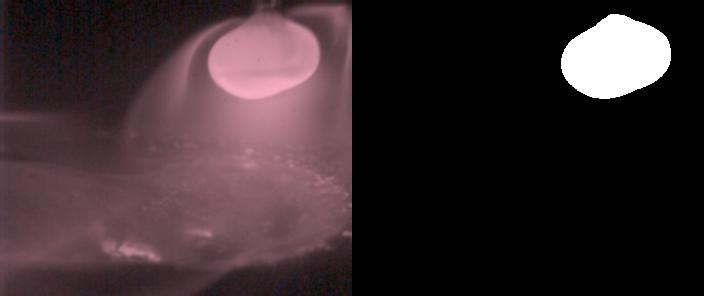
\includegraphics[width=\linewidth]{Images/Results/glob_pred_0.jpg}
    \caption{}

  \end{subfigure}
\hfill
  \begin{subfigure}[b]{0.45\textwidth}
    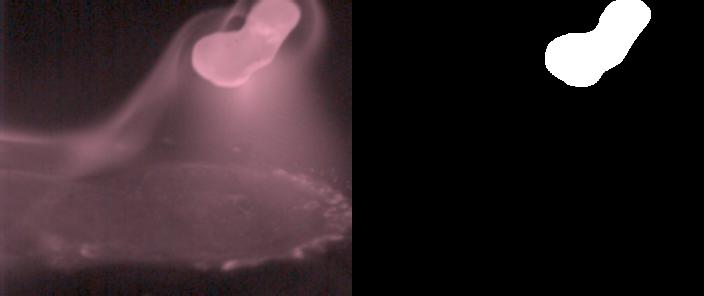
\includegraphics[width=\linewidth]{Images/Results/glob_pred_3870.jpg}
    \caption{}

  \end{subfigure}
  \begin{subfigure}[b]{0.45\textwidth}
    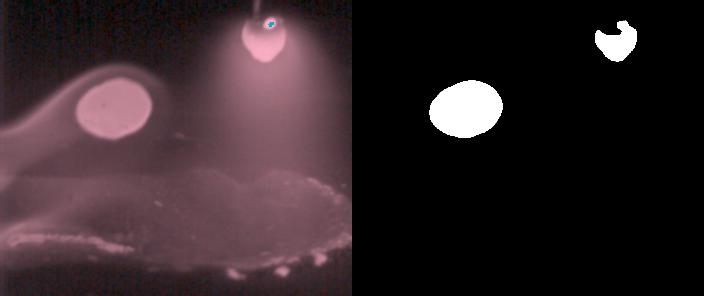
\includegraphics[width=\linewidth]{Images/Results/glob_pred_4817.jpg}
    \caption{}

  \end{subfigure}
    \caption[Globular transfer mode predictions]{Globular transfer mode predictions.}
    \label{fig:glob_pred_samples}
\end{figure}

\begin{figure}
\centering
  \begin{subfigure}[b]{0.45\textwidth}
    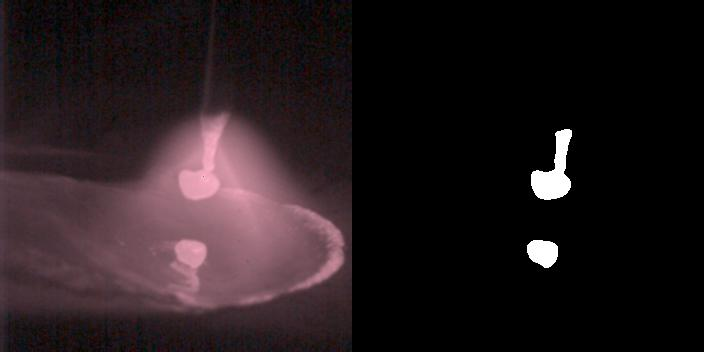
\includegraphics[width=\linewidth]{Images/Results/spray_pred_15.jpg}
    \caption{}

  \end{subfigure}
\hfill
  \begin{subfigure}[b]{0.45\textwidth}
    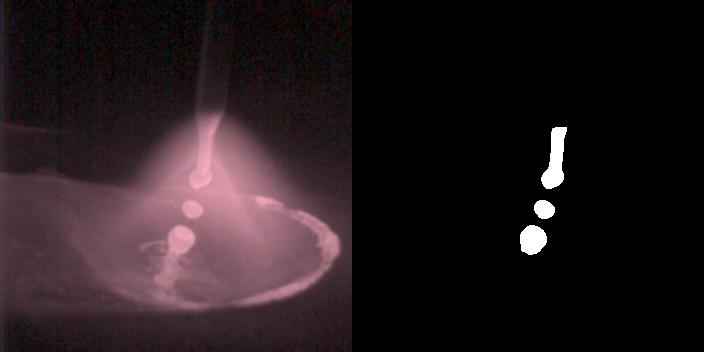
\includegraphics[width=\linewidth]{Images/Results/spray_pred_1937.jpg}
    \caption{}

  \end{subfigure}
  \begin{subfigure}[b]{0.45\textwidth}
    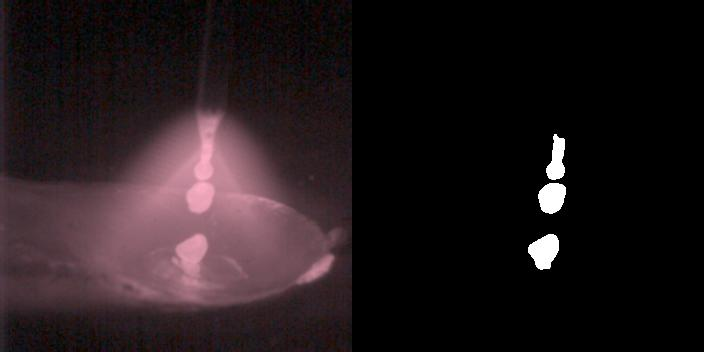
\includegraphics[width=\linewidth]{Images/Results/spray_pred_3269.jpg}
    \caption{}

  \end{subfigure}
    \caption[Spray transfer mode predictions]{Spray transfer mode predictions.}
    \label{fig:spray_pred_samples}
\end{figure}

Moreover, an important aspect of this work is that the labels were manually generated, so the results are subject to a human bias, specifically the selection of the boundary of the droplet because at a pixel level there is not an exact distinction between droplet and background and a gradient is seen between the brighter pixels of the droplet and the darker pixels of the background. Hence, to make more evident where the network decides to make  the droplet-background division which is influenced by the labeling, figures \ref{fig:boundary_globular} and \ref{fig:boundary_spray} show the pixel values of a single horizontal strip, specifically the one that goes through the centroid of the droplet segmentation. There, one can see that there is a transition between droplet and background, and vertical lines show where the model cuts and makes the segmentation. The figures show that in the image there there is a steep transition between background and droplet, and the segmentation cuts around the middle of that transition.


\begin{figure}
    \centering
    \import{Images/Results/boundary_globular/}{500.pgf}
    \caption[Boundary predicted by the model with respect to original globular image]{Boundary predicted by the model with respect to original globular image. A horizontal strip is taken along the droplet's centroid (dashed yellow line in (a) and (b)) and the pixel values along that line are shown in (c). In (b) the predicted mask which generates the red curve in (c) is shown.}
    \label{fig:boundary_globular}
\end{figure}

\begin{figure}
    \centering
    \import{Images/Results/boundary_spray/}{500.pgf}
    \caption[Boundary predicted by the model with respect to original spray image]{Boundary predicted by the model with respect to original spray image.}
    \label{fig:boundary_spray}
\end{figure}


\clearpage
\section{Post processing}

\begin{figure}
\centering
  \begin{subfigure}[b]{0.45\textwidth}
    \import{Images/Results/centroid_samples/}{globular_0.pgf}
    \caption{}

  \end{subfigure}
\hfill
  \begin{subfigure}[b]{0.45\textwidth}
    \import{Images/Results/centroid_samples/}{globular_790.pgf}
    \caption{}
  \end{subfigure}
  \begin{subfigure}[b]{0.45\textwidth}
    \import{Images/Results/centroid_samples/}{globular_2360.pgf}
    \caption{}
  \end{subfigure}
    \caption[Spray transfer mode predictions]{Spray transfer mode predictions.}
    \label{fig:globular_centroids}
\end{figure}

\begin{figure}
\centering
  \begin{subfigure}[b]{0.45\textwidth}
    \import{Images/Results/centroid_samples/}{spray_0.pgf}
    \caption{}

  \end{subfigure}
\hfill
  \begin{subfigure}[b]{0.45\textwidth}
    \import{Images/Results/centroid_samples/}{spray_42.pgf}
    \caption{}
  \end{subfigure}
  \begin{subfigure}[b]{0.45\textwidth}
    \import{Images/Results/centroid_samples/}{spray_656.pgf}
    \caption{}
  \end{subfigure}
    \caption[Spray transfer mode predictions]{Spray transfer mode predictions.}
    \label{fig:spray_centroids}
\end{figure}
